\section{Results}
\label{sec:results}

Everything below is measured in one harness (\texttt{run\_bench.py}) with the same seed program,
the same evaluator and the same budgets for every method; the four methods differ only in how
they spend the budget. Three arms (\texttt{--seed 0/1/2}) per method and task; the seed only
drives the method's own draws (parents, inspirations, ideas) --- the model's sampling is not
seeded, so arms are independent runs, not a paired design. A finished arm reports its best
program's \emph{first} full-fidelity read; a still-running arm ($^\circ$ in the tables, hollow in
the figures) reports its best so far, a lower bound.

\begin{center}\small
\begin{tabular}{@{}>{\raggedright\arraybackslash}p{24mm}>{\raggedright\arraybackslash}p{44mm}>{\raggedright\arraybackslash}p{34mm}>{\raggedright\arraybackslash}p{46mm}@{}}
\toprule
& AHC039 & circle packing $n{=}26$ & Erd\H{o}s minimum overlap \\
\midrule
score & official points per case (mean of 150 cases, 2 s each) & sum of radii & $\Psi$, lower is better \\
seed program & a 5th-place contest solution ($\approx$3700) & a plain grid (1.8045) & uniform ($\Psi=0.5$) \\
evaluation rule & shared eval server, C++ time limits & feasibility to $10^{-12}$ & 120 s from scratch, no warm start \\
reference & --- & record 2.635983 & 0.380909 (ours, earlier) / 0.380924 (AlphaEvolve) \\
LLM budget & 480 calls (no token cap) & 160 calls, 3.5 M tokens & 160 calls, 3.5 M tokens \\
evaluator budget & 500 calls & 100 calls & 150 calls \\
\bottomrule
\end{tabular}
\end{center}

\noindent Models: \texttt{deepseek-v4-flash} (the flash campaign, \S\ref{sec:flash}) and
\texttt{deepseek-v4-pro-0813} (\S\ref{sec:pro}), both through OpenRouter at 64k output tokens.
The pro campaign used the same budgets with two workers instead of four; its AHC039 arms ran on a
separate eval server.

\subsection{Flash campaign: three tasks, four methods}
\label{sec:flash}

\begin{table}[H]\centering\small
\caption{deepseek-v4-flash, all 36 arms finished. Best per arm (s0 / s1 / s2), method mean, and mean
LLM tokens spent (millions). SimpleTES's AHC039 s1/s2 and packing s1 were restarted after Modal
preemptions and resumed from checkpoints; their token figures include the interrupted runs.}
\label{tab:flash}
\begin{tabular}{@{}lrrrrr@{}}
\toprule
\multicolumn{6}{@{}l}{\textbf{AHC039} --- official points per case, higher is better} \\
method & s0 & s1 & s2 & mean & tokens \\
\midrule
HypothesisBandit & 3724 & 3714 & 3730 & 3723 & 15.8 \\
AgentMapElites & 3709 & 3726 & 3723 & 3719 & 16.5 \\
SimpleTES & 3712 & 3700 & 3722 & 3711 & 25.8 \\
\textbf{LabNotebook} & \textbf{3744} & 3722 & 3733 & \textbf{3733} & 17.4 \\
\midrule
\multicolumn{6}{@{}l}{\textbf{circle packing $n{=}26$} --- sum of radii, record 2.635983} \\
\midrule
HypothesisBandit & 2.635896 & 2.615307 & 2.622878 & 2.624694 & 3.3 \\
AgentMapElites & 1.804524 & 1.804524 & 2.433600 & 2.014216 & 3.8 \\
SimpleTES & 2.634292 & 2.635983 & 2.634293 & 2.634856 & 3.4 \\
\textbf{LabNotebook} & \textbf{2.635983} & \textbf{2.635983} & \textbf{2.635983} & \textbf{2.635983} & 3.4 \\
\midrule
\multicolumn{6}{@{}l}{\textbf{Erd\H{o}s} --- $\Psi$, lower is better, record 0.380909} \\
\midrule
HypothesisBandit & 0.387629 & 0.382043 & 0.382516 & 0.384063 & 3.2 \\
AgentMapElites & 0.383916 & 0.500000 & 0.381835 & 0.421917 & 3.7 \\
SimpleTES & 0.381340 & 0.381359 & 0.381293 & 0.381331 & 3.6 \\
\textbf{LabNotebook} & \textbf{0.381031} & 0.381077 & 0.381411 & \textbf{0.381173} & 3.5 \\
\bottomrule
\end{tabular}
\end{table}

\begin{figure}[H]\centering
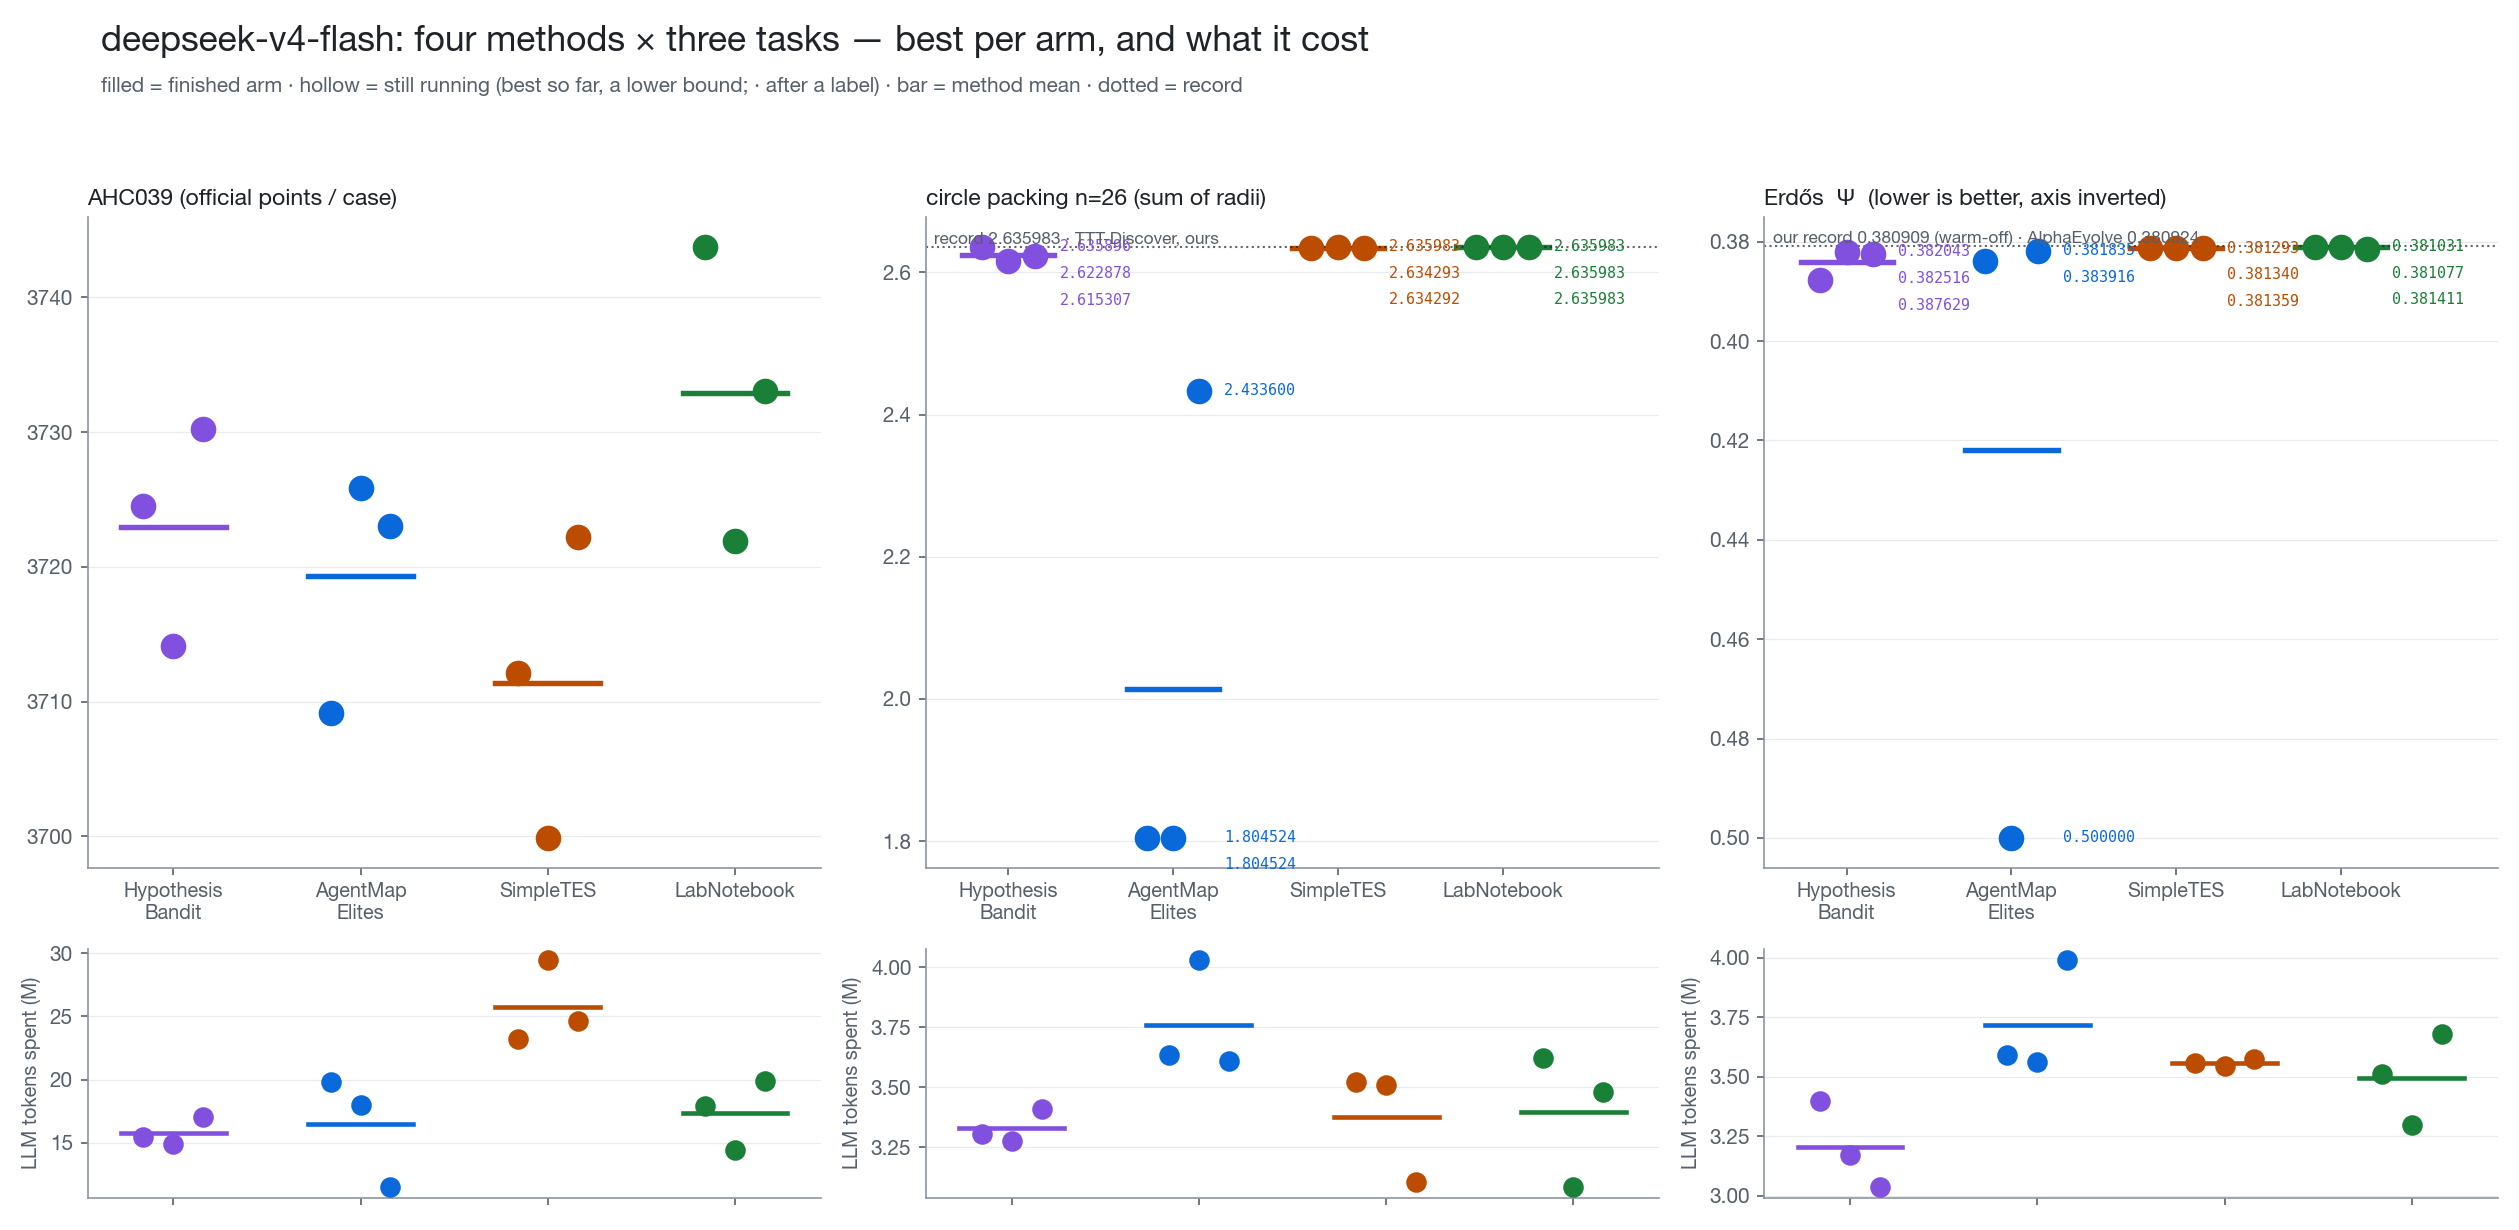
\includegraphics[width=\textwidth]{lab_notebook_figs/overview_flash.png}
\caption{Flash campaign, all arms finished: one marker per arm, bar = method mean, dotted = record; the
lower row is what each arm spent. LabNotebook holds the best mean on all three tasks, the record on
3/3 packing arms (SimpleTES 1/3), and the tightest replicate spread.}
\end{figure}

\begin{figure}[H]\centering
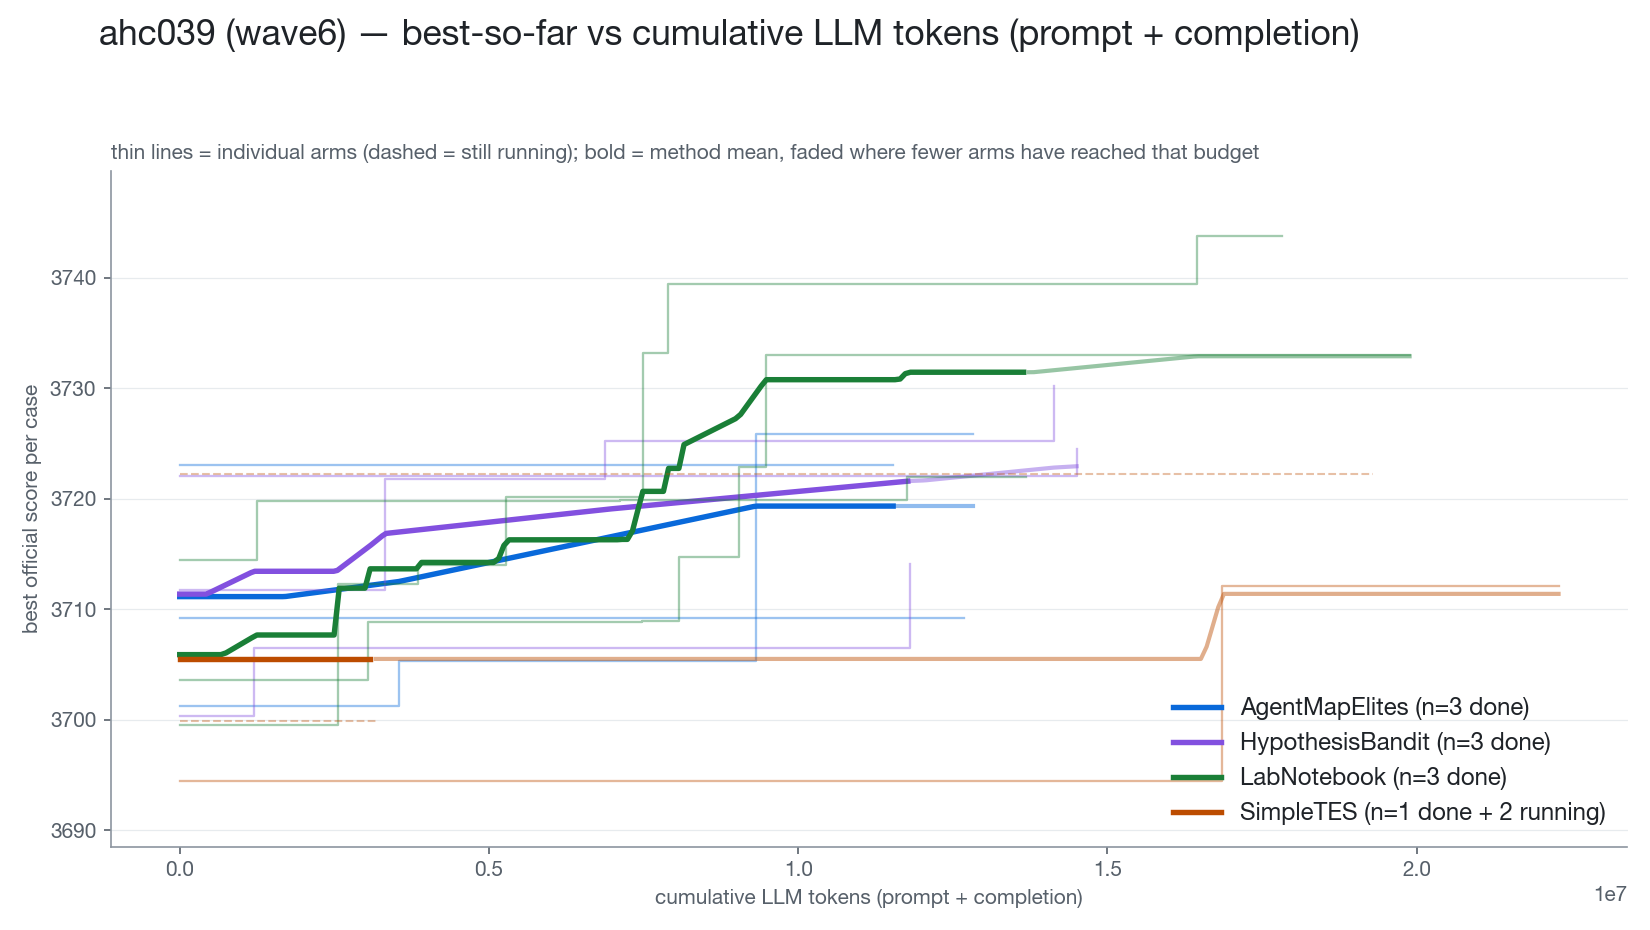
\includegraphics[width=\textwidth]{lab_notebook_figs/budget_tokens_ahc039_flash.png}
\caption{AHC039, flash: best-so-far against cumulative LLM tokens. LabNotebook's curve rises in
steps --- each step is a cycle whose best trajectory beat the champion --- and keeps rising past
10~M tokens where the other methods have flattened.}
\end{figure}

\subsection{Pro campaign}
\label{sec:pro}

\begin{table}[H]\centering\small
\caption{deepseek-v4-pro-0813, same budgets, all 36 arms finished. AHC039 ran on its own eval server,
so its points are comparable within this table, not with Table~\ref{tab:flash}. The SimpleTES AHC039
arms were preempted repeatedly and resumed; s2 was once restarted from scratch under the pre-resume
launcher and lost 197 calls. Their token figures include the interrupted runs.}
\label{tab:pro}
\begin{tabular}{@{}lrrrrr@{}}
\toprule
\multicolumn{6}{@{}l}{\textbf{AHC039}} \\
method & s0 & s1 & s2 & mean & tokens \\
\midrule
HypothesisBandit & 3707 & 3708 & 3706 & 3707 & 15.3 \\
AgentMapElites & 3721 & 3724 & 3703 & 3716 & 17.6 \\
SimpleTES & 3704 & 3712 & 3711 & 3709 & 35.0 \\
\textbf{LabNotebook} & 3747 & 3759 & \textbf{3776} & \textbf{3761} & 20.4 \\
\midrule
\multicolumn{6}{@{}l}{\textbf{circle packing $n{=}26$}} \\
\midrule
HypothesisBandit & 2.627800 & 2.622606 & 2.631937 & 2.627448 & 3.1 \\
AgentMapElites & 2.630175 & 2.630058 & 2.635983 & 2.632072 & 3.9 \\
SimpleTES & 2.635983 & 2.635983 & 2.634292 & 2.635420 & 3.6 \\
LabNotebook & 2.634292 & 2.635985$^\dagger$ & 2.635983 & 2.635420 & 3.3 \\
\midrule
\multicolumn{6}{@{}l}{\textbf{Erd\H{o}s}} \\
\midrule
HypothesisBandit & 0.381893 & \textbf{0.380981} & 0.382323 & 0.381732 & 3.5 \\
AgentMapElites & 0.381450 & 0.381243 & 0.381165 & 0.381286 & 3.6 \\
SimpleTES & 0.381181 & 0.381205 & 0.381065 & 0.381150 & 3.6 \\
\textbf{LabNotebook} & 0.381139 & 0.381118 & 0.381081 & \textbf{0.381113} & 3.5 \\
\bottomrule
\end{tabular}

\smallskip\footnotesize $^\dagger$ 2.635985 exceeds the record only through the verifier's
$10^{-12}$ tolerance; at zero tolerance it is 2.635983.
\end{table}

\begin{figure}[H]\centering
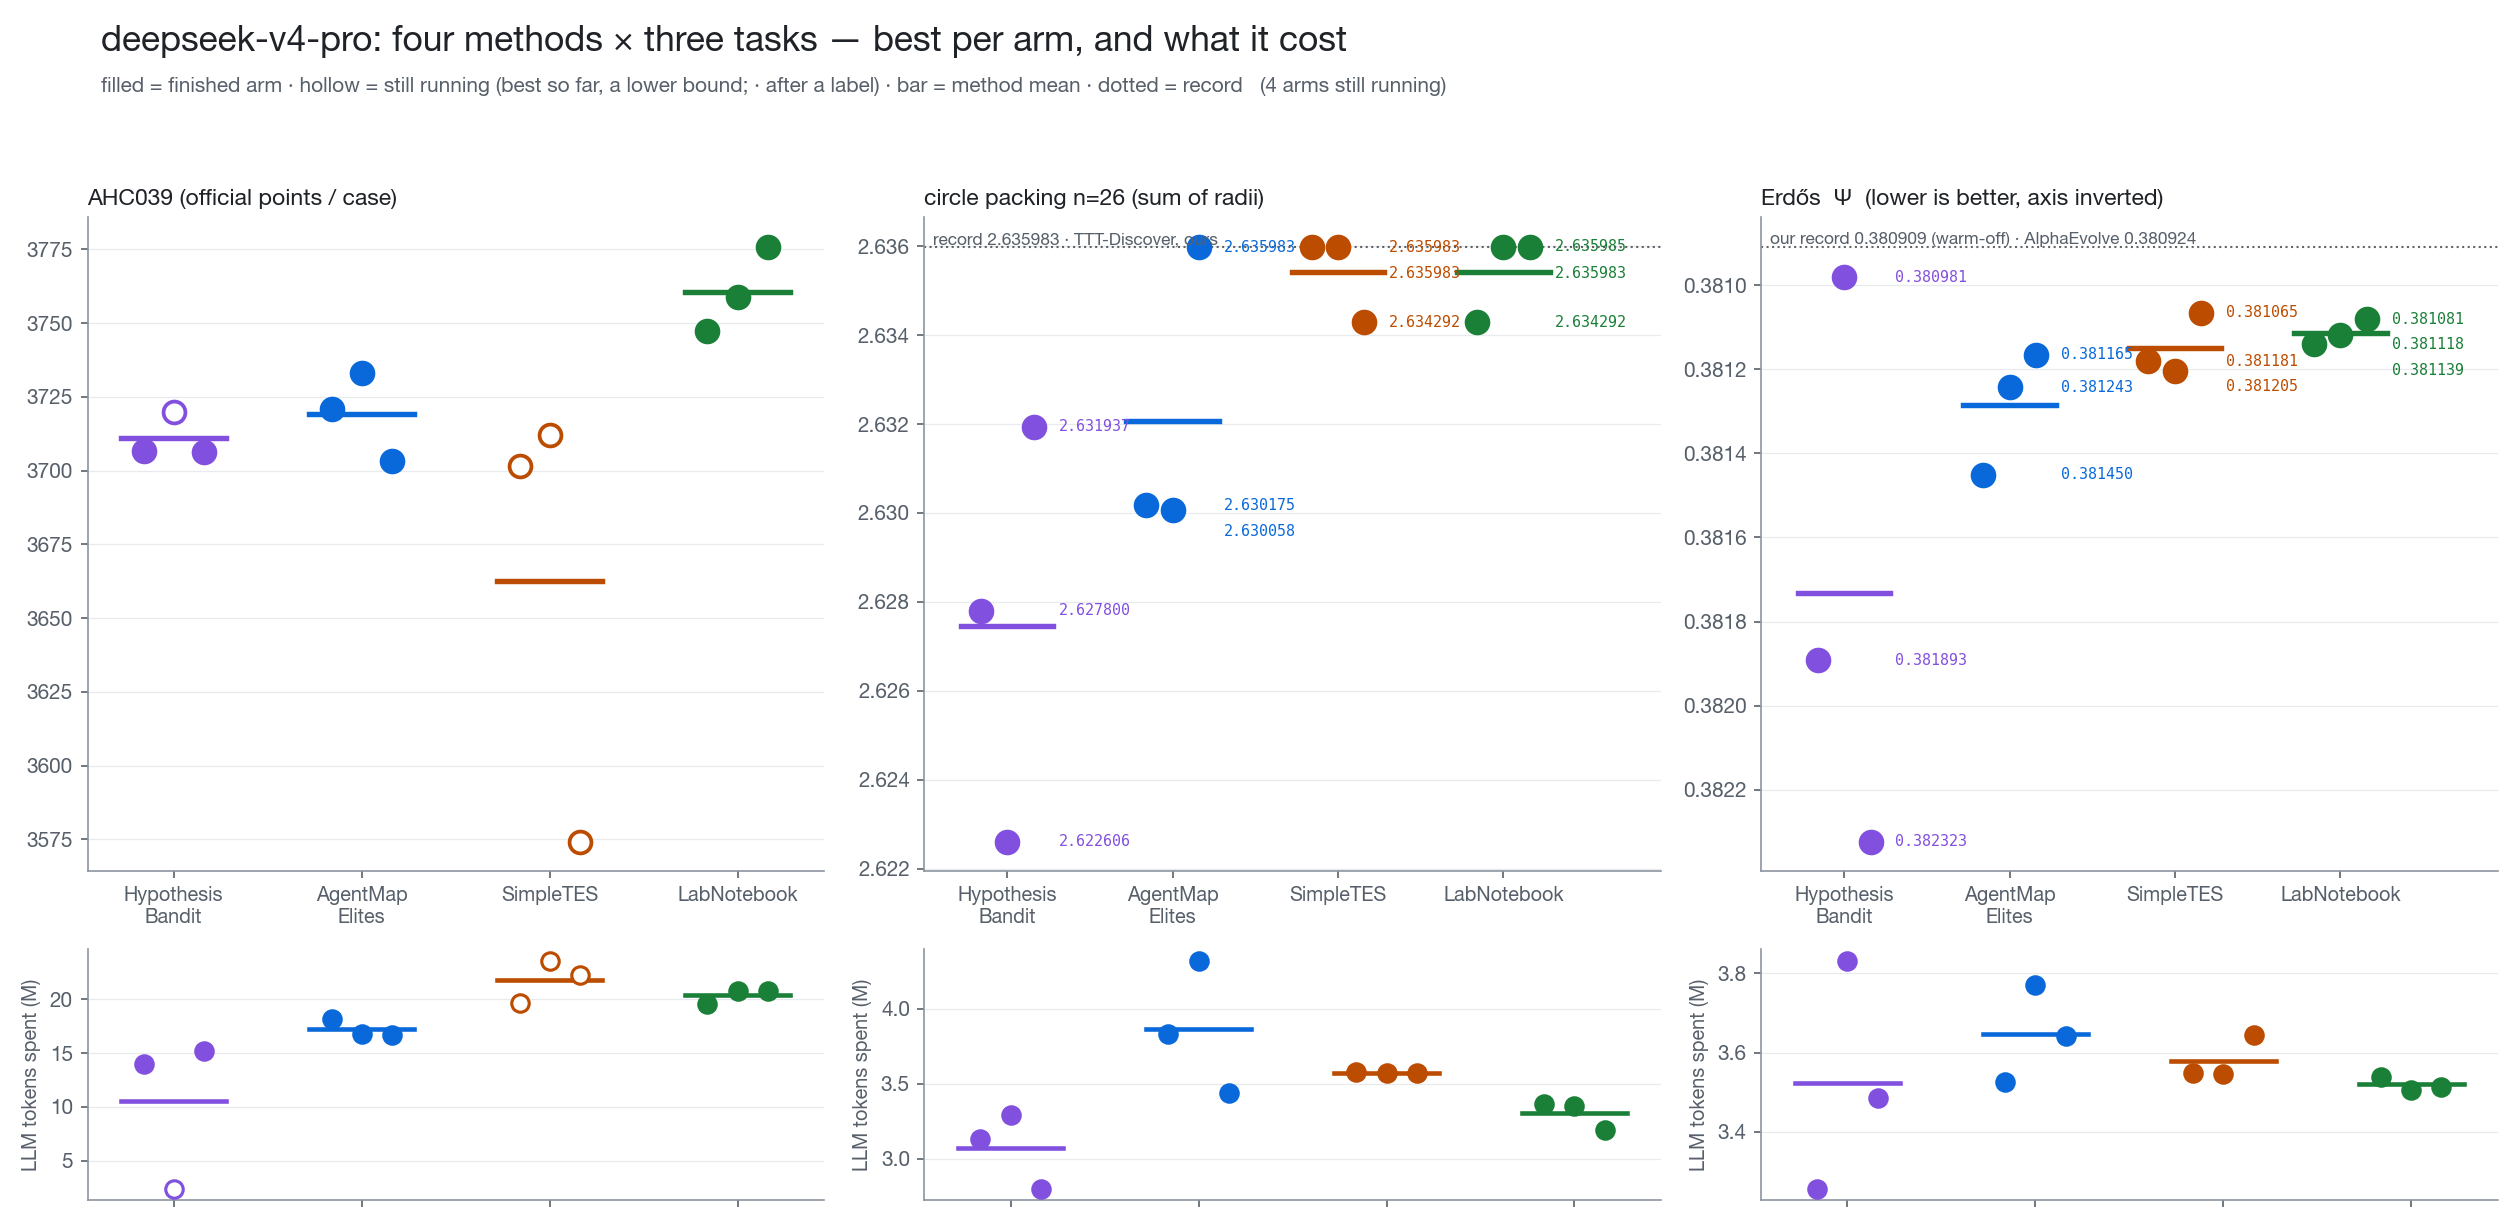
\includegraphics[width=\textwidth]{lab_notebook_figs/overview_pro.png}
\caption{Pro campaign, all arms finished. On AHC039 every LabNotebook arm is above every arm of every
other method (next best: MAP-Elites 3724; SimpleTES 3712); 3776 is the best score of both campaigns. Packing and Erd\H{o}s are ties within
replicate spread --- both are problems where the answer is a known local optimum that any good
inner optimizer reaches.}
\end{figure}

\begin{figure}[H]\centering
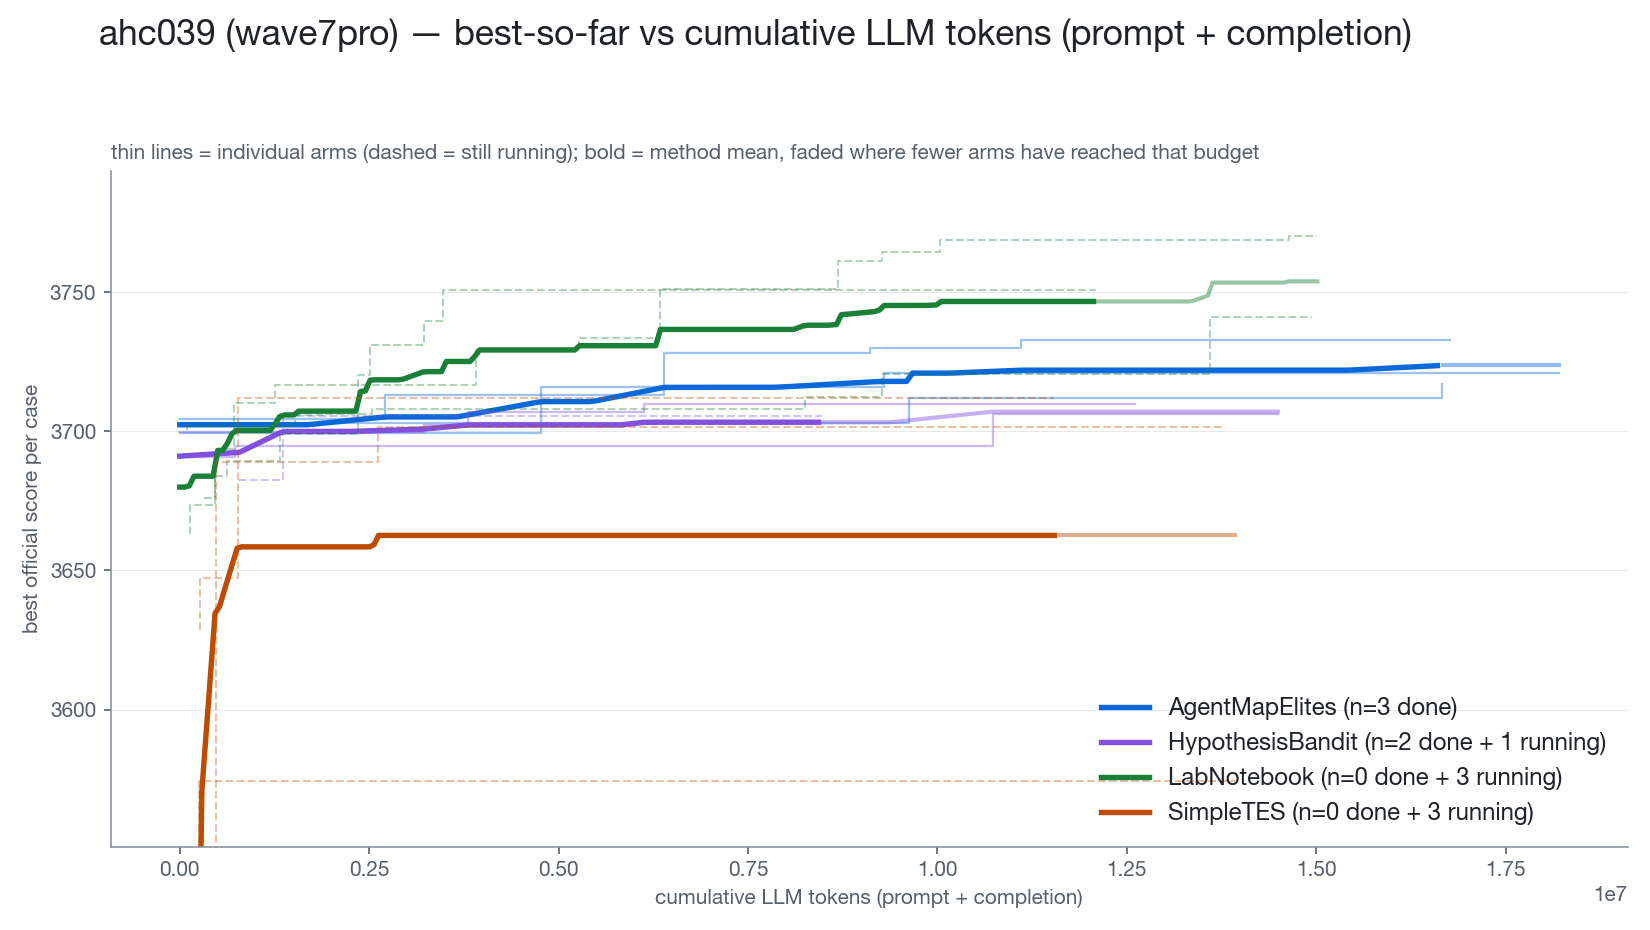
\includegraphics[width=\textwidth]{lab_notebook_figs/budget_tokens_ahc039_pro.png}
\caption{AHC039, pro: best-so-far against cumulative LLM tokens.}
\end{figure}

\subsection{Erd\H{o}s: the 0.381 floor, and two ways past it}

\begin{figure}[H]\centering
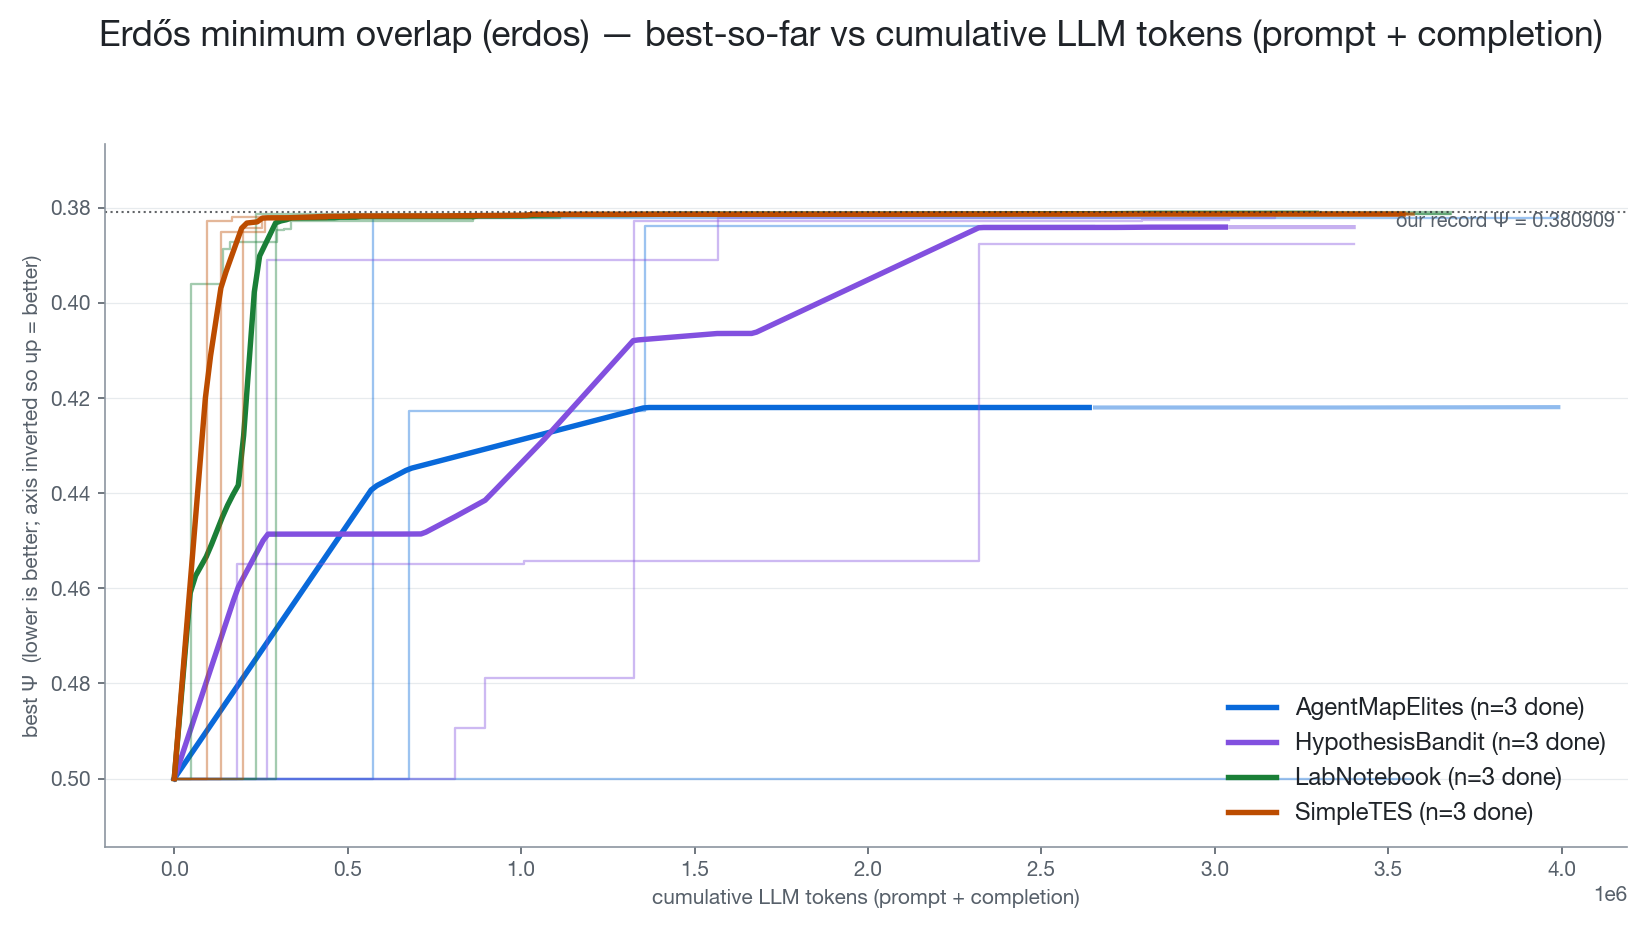
\includegraphics[width=\textwidth]{lab_notebook_figs/budget_tokens_erdos_flash.png}
\caption{Erd\H{o}s, flash: every method converges to $\Psi\approx0.381$ and stops. The barrier
is the evaluation rule, not the search: a construction is rebuilt from scratch in 120 s, and at
the discretisation that fits in 120 s the local minimax optima sit at 0.381. The published
0.3809 values were reached by accumulating polish across many runs.}
\end{figure}

\paragraph{Protocol A --- search, then equal polish.} Each method's best \emph{construction}
was given the same fixed block-coordinate SLP polisher, in rounds of $\le 120$ s, so the comparison
measures the shape the search found rather than the optimizer its program contained.

\begin{center}\small
\begin{tabular}{@{}lrrl@{}}
\toprule
method & search ($\Psi$) & after polish & note \\
\midrule
LabNotebook & 0.381032 & 0.381032 & no round improved it: already a local minimax optimum \\
SimpleTES & 0.381293 & 0.381060 & \\
HypothesisBandit & 0.382044 & 0.381348 & \\
AgentMapElites & 0.381880 & 0.381639 & \\
\bottomrule
\end{tabular}
\end{center}

\begin{figure}[H]\centering
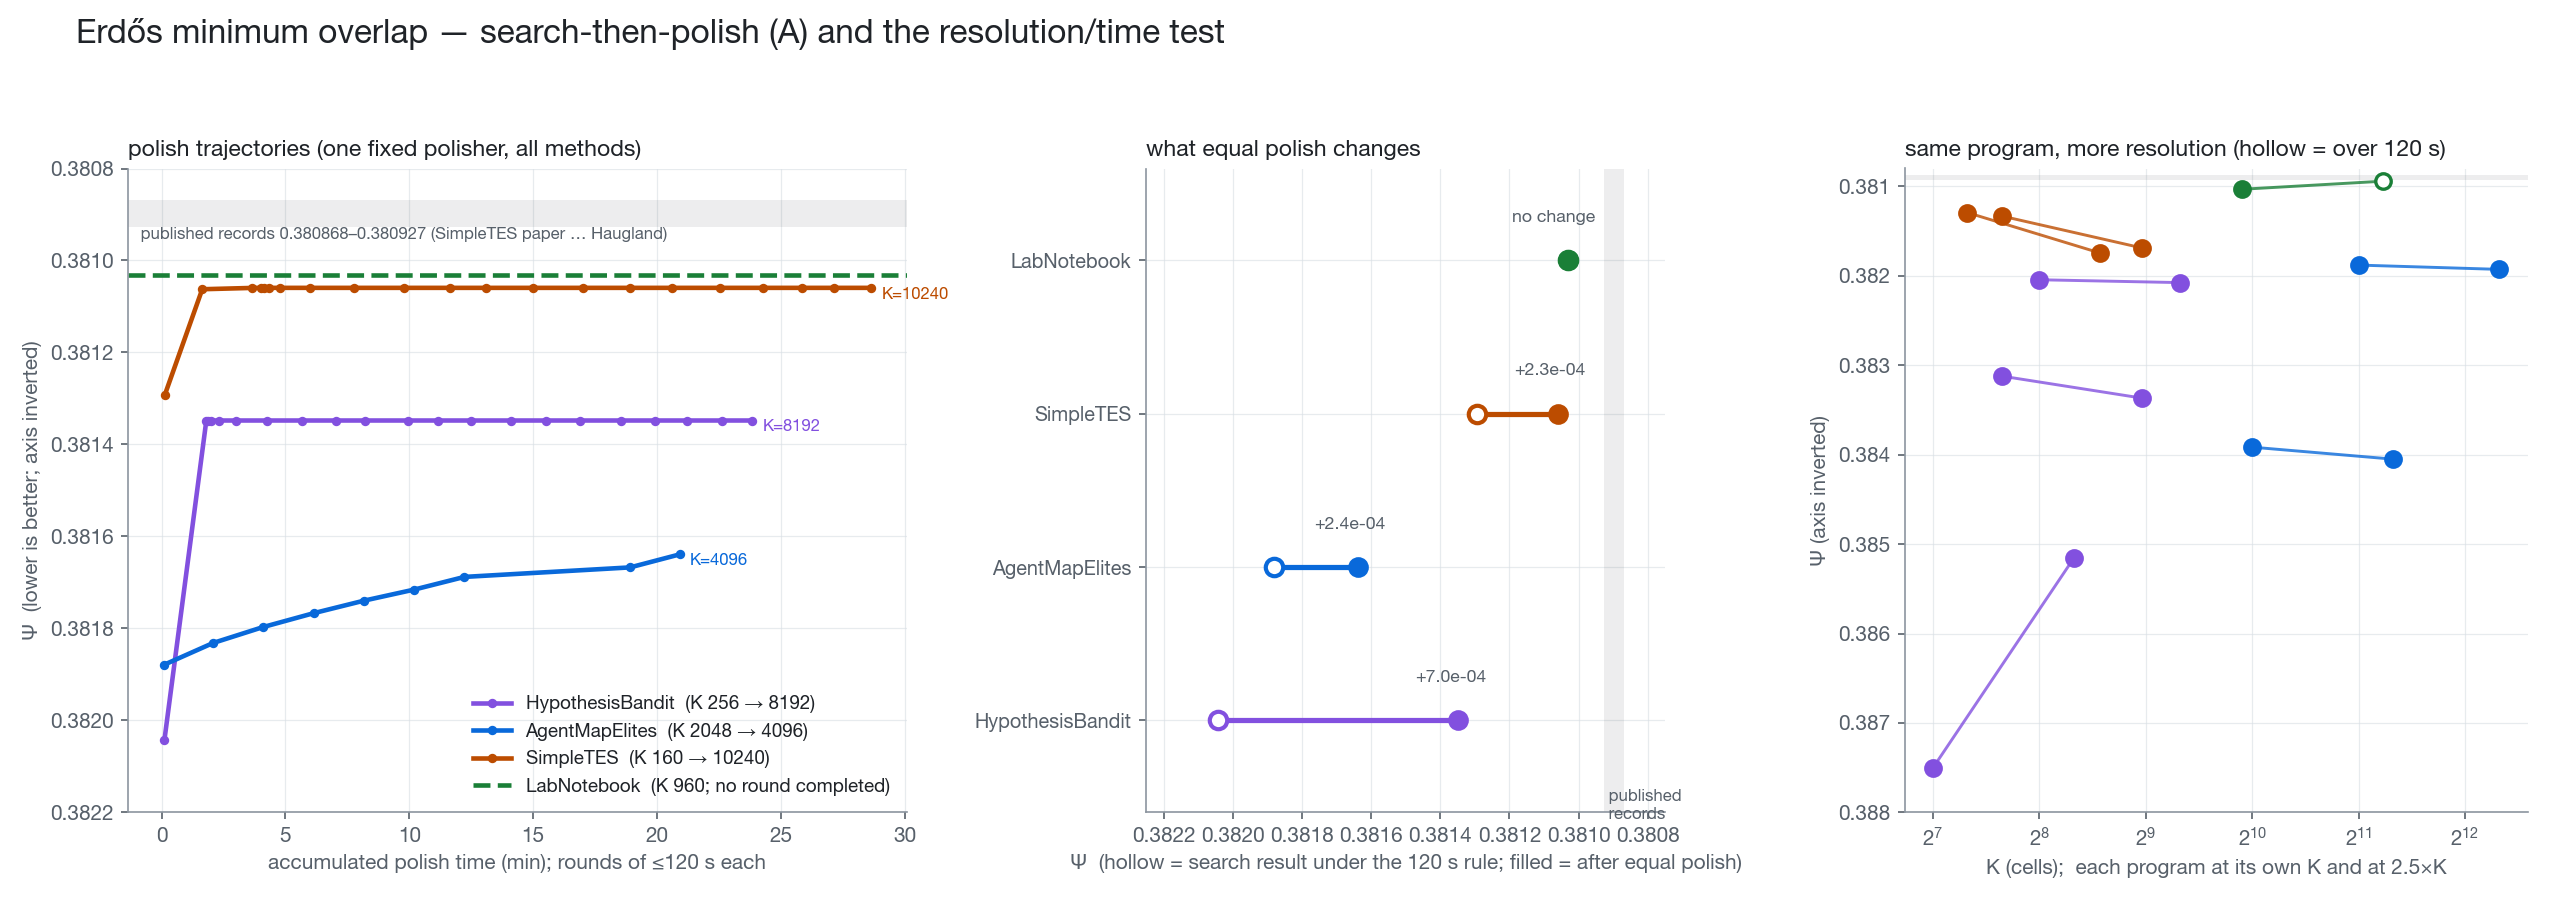
\includegraphics[width=\textwidth]{lab_notebook_figs/polish_erdos.png}
\caption{Protocol A: polish trajectories (left), search $\to$ polished (middle), and the same
program re-run at $2.5\times$ its resolution under a 500 s cap (right). Only LabNotebook's
program benefits from more resolution ($0.380942$ at $K{=}2400$); the others' constructions are
local optima at any resolution.}
\end{figure}

\paragraph{Protocol B --- a persisted warm start.} The Erd\H{o}s wave re-run with each arm's
best construction persisted between evaluations (the published records' setting). This is the one
setting where SimpleTES beats LabNotebook: given a good incumbent, SimpleTES's exploit-heavy
chain polishes it, while LabNotebook keeps spending trajectories on new ideas.

\begin{table}[H]\centering\small
\caption{Protocol B (flash). Warm-start $\Psi$ per arm and mean; the last column is the same
method's cold-start mean from Table~\ref{tab:flash}.}
\begin{tabular}{@{}lrrrrr@{}}
\toprule
method & s0 & s1 & s2 & mean (warm) & mean (cold) \\
\midrule
HypothesisBandit & 0.383857 & 0.381503 & 0.396447 & 0.387269 & 0.384063 \\
AgentMapElites & 0.381143 & 0.500000 & \textbf{0.380999} & 0.420714 & 0.421917 \\
SimpleTES & 0.381051 & 0.381075 & 0.381005 & \textbf{0.381044} & 0.381331 \\
LabNotebook & \textbf{0.380999} & 0.381341 & 0.382348 & 0.381563 & 0.381173 \\
\bottomrule
\end{tabular}
\end{table}

\begin{figure}[H]\centering
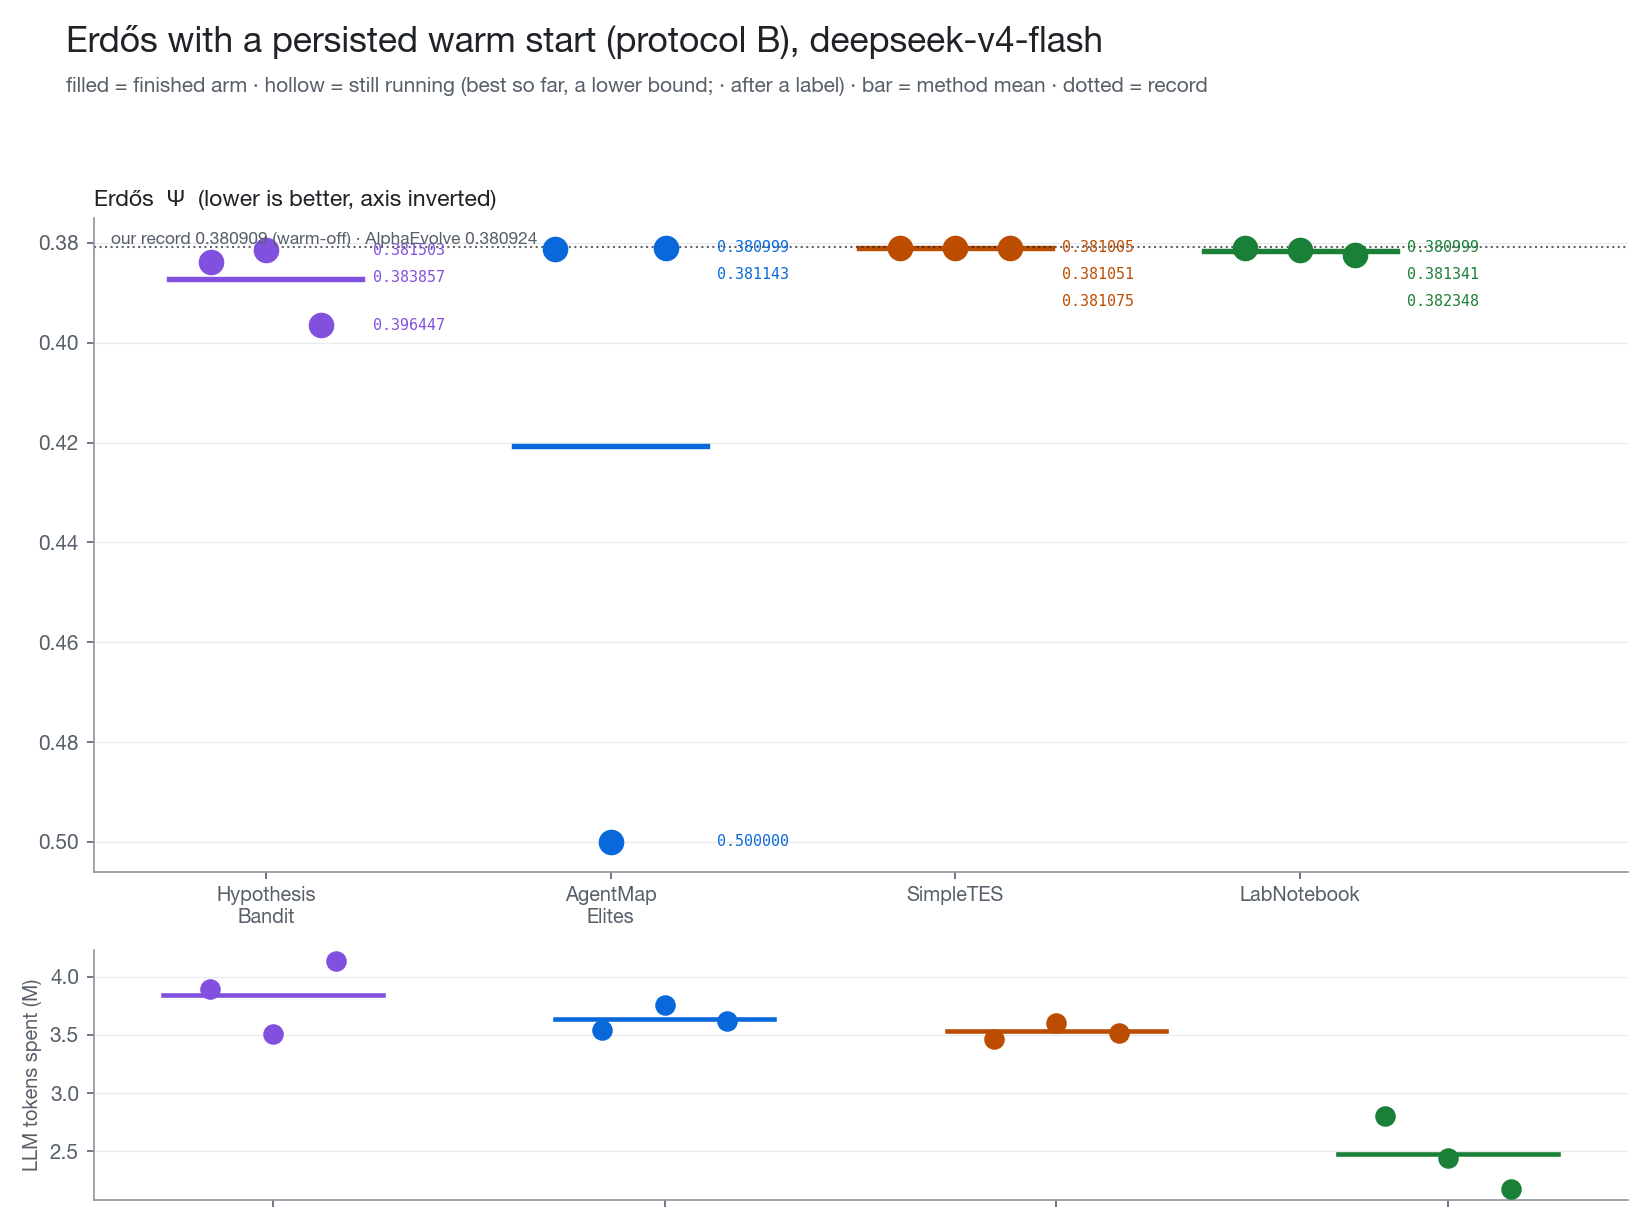
\includegraphics[width=0.85\textwidth]{lab_notebook_figs/overview_erdos_warm.png}
\caption{Protocol B, per arm. Two arms reach 0.380999, the first values below 0.381 in this
harness; the 0.380909 record was not reached by any method under either protocol.}
\end{figure}

\subsection{AlphaEvolve-suite tasks, batch A}
\label{sec:ae}

Three tasks from the AlphaEvolve suite under SimpleTES's task contract, run with our model
(\texttt{deepseek-v4-flash}) and harness at 160 LLM calls, 3.5 M tokens and 100 evaluations
(60 for the autocorrelation tasks) per arm, with a 300 s evaluation cap. The published systems
used different models and two to three orders of magnitude more compute (TTT-Discover: gpt-oss-120b,
$50\times512$ rollouts, $\approx\$500$ per run; ThetaEvolve: $\approx$300k programs; SimpleTES:
gpt-oss-120b with an 1100 s evaluation cap), so their numbers are context, not competitors. The
harness score for $C_1$ is $1/C_1$; the table reports $C_1$ itself.

\begin{table}[H]\centering\small
\caption{Batch A, all 36 arms finished: per-arm results in the papers' units, with the published values.}
\label{tab:ae}
\begin{tabular}{@{}lrrrrr@{}}
\toprule
\multicolumn{6}{@{}l}{\textbf{circle packing $n{=}32$} --- sum of radii, higher is better} \\
method & s0 & s1 & s2 & mean & tokens \\
\midrule
HypothesisBandit & 1.722894 & 2.751149 & 2.395420 & 2.289821 & 3.3 \\
AgentMapElites & 2.515664 & 2.918279 & 2.474720 & 2.636221 & 3.8 \\
SimpleTES & 2.939573 & 2.933651 & 2.939573 & 2.937599 & 3.6 \\
\textbf{LabNotebook} & \textbf{2.939573} & \textbf{2.939573} & \textbf{2.939573} & \textbf{2.939573} & 3.5 \\
\multicolumn{6}{@{}l}{\footnotesize published: best human 2.936 $\cdot$ AlphaEvolve v1 2.937944 $\cdot$ record 2.939572} \\
\multicolumn{6}{@{}l}{\footnotesize \phantom{published: }(AlphaEvolve V2, TTT-Discover, SimpleTES)} \\
\midrule
\multicolumn{6}{@{}l}{\textbf{$C_1$, first autocorrelation inequality} --- upper bound, lower is better} \\
\midrule
HypothesisBandit & 1.51453 & 1.51589 & 1.51589 & 1.51544 & 3.4 \\
AgentMapElites & 1.51589 & 1.51450 & 1.51273 & 1.51437 & 3.7 \\
\textbf{SimpleTES} & \textbf{1.50941} & 1.51148 & 1.51088 & \textbf{1.51059} & 2.6 \\
LabNotebook & 1.51063 & 1.51267 & 1.50947 & 1.51093 & 2.2 \\
\multicolumn{6}{@{}l}{\footnotesize published: best human 1.50973 $\cdot$ AlphaEvolve v1 1.5053 $\cdot$ ThetaEvolve 1.50314} \\
\multicolumn{6}{@{}l}{\footnotesize \phantom{published: }AlphaEvolve V2 1.50317 $\cdot$ TTT-Discover 1.50287 (record)} \\
\midrule
\multicolumn{6}{@{}l}{\textbf{$C_2$, second autocorrelation inequality} --- lower bound, higher is better} \\
\midrule
HypothesisBandit & 0.9098 & 0.9057 & 0.9062 & 0.9072 & 3.9 \\
AgentMapElites & 0.9127 & 0.9086 & 0.9088 & 0.9100 & 4.1 \\
SimpleTES & 0.9101 & 0.9079 & 0.9139 & 0.9106 & 3.1 \\
\textbf{LabNotebook} & \textbf{0.9248} & 0.9106 & 0.9185 & \textbf{0.9180} & 2.2 \\
\multicolumn{6}{@{}l}{\footnotesize published: best human 0.9015 $\cdot$ AlphaEvolve v1 0.8962 $\cdot$ ThetaEvolve 0.9469} \\
\multicolumn{6}{@{}l}{\footnotesize \phantom{published: }TTT-Discover 0.9591 $\cdot$ AlphaEvolve V2 0.9610 $\cdot$ SimpleTES 0.9627 (record)} \\
\bottomrule
\end{tabular}
\end{table}

\begin{figure}[H]\centering
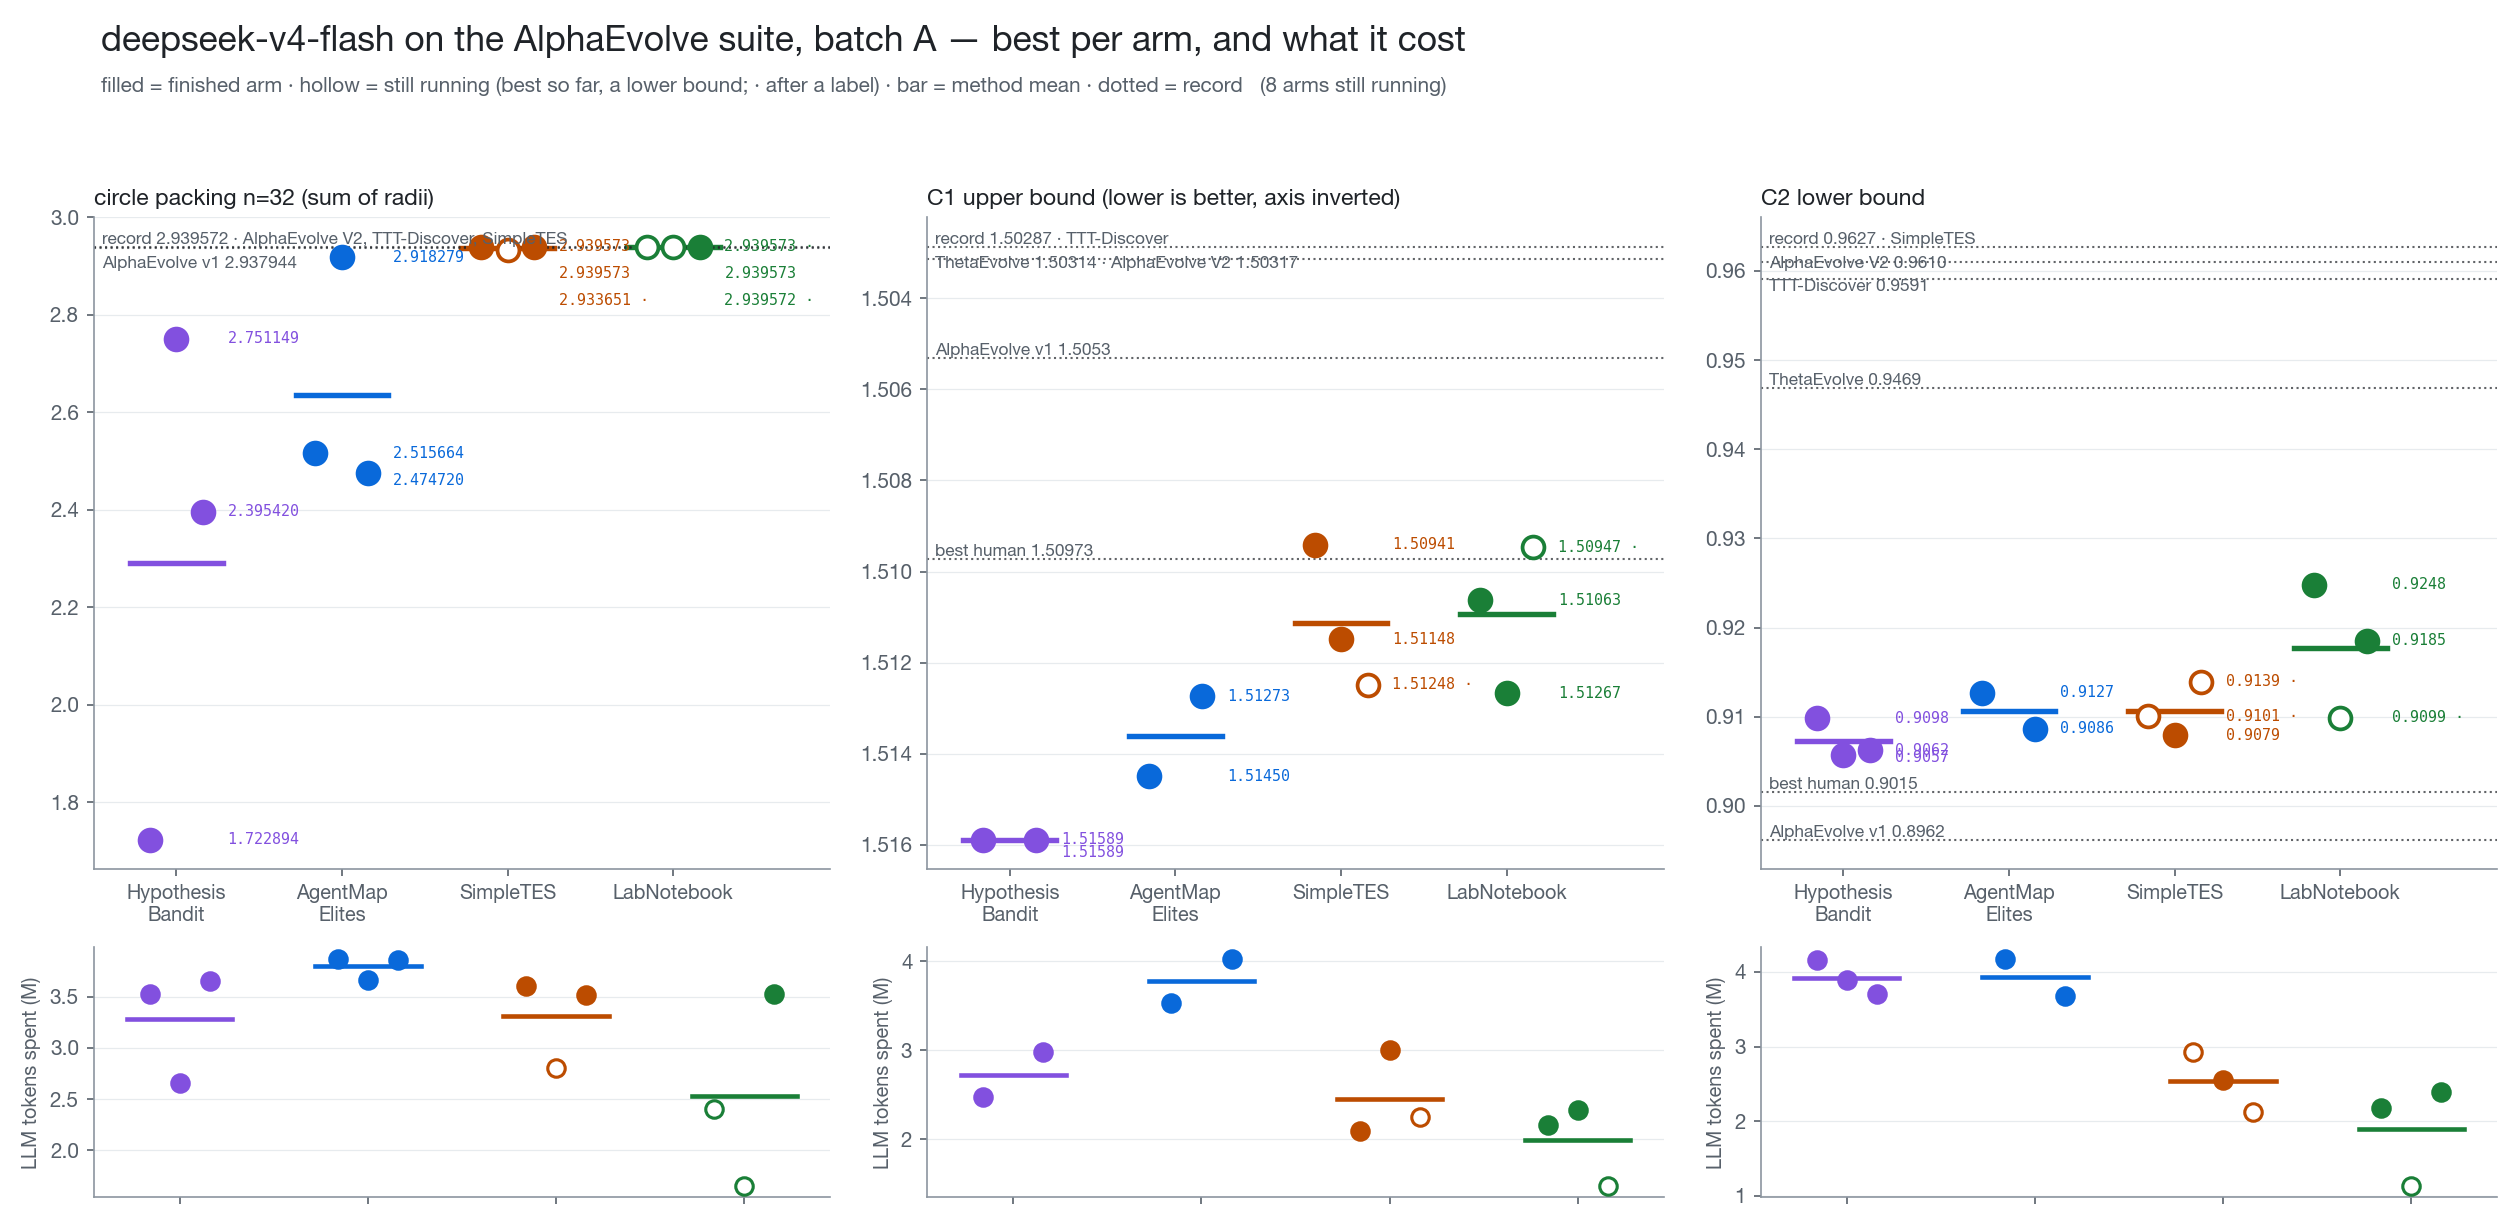
\includegraphics[width=\textwidth]{lab_notebook_figs/overview_ae_batchA.png}
\caption{Batch A with every published bound drawn. Packing $n{=}32$: five arms sit on the record
(LabNotebook 3/3, SimpleTES 2/3). $C_1$: the best arms fall between the human record and AlphaEvolve
v1, with the 2026 systems a clear band above. $C_2$: above AlphaEvolve v1 and the human best, well
below the 2026 band.}
\end{figure}

\paragraph{Batch B.} Third autocorrelation inequality ($C_3$, upper bound, lower is
better; harness score $1.4556/C_3$), sums vs differences ($C(A)$, higher is better) and the
Hadamard maximal determinant of order 29 (score $|\det|$ relative to a reference; no published
value recorded). Published: $C_3$ --- AlphaEvolve 1.4556, TTT-Discover 1.454555, SimpleTES 1.453675
(record); $C(A)$ --- SimpleTES 1.1449. All 36 arms finished. The MAP-Elites $C_3$ construction re-evaluates to exactly
1.453675 --- SimpleTES's published value to six decimals --- so the model reproduced the known
construction rather than finding a new one; it is reported but not claimed.

\begin{table}[H]\centering\small
\caption{Batch B, all 36 arms finished: per-arm results in the papers' units.}
\label{tab:aeb}
\begin{tabular}{@{}lrrrrr@{}}
\toprule
\multicolumn{6}{@{}l}{\textbf{$C_3$, third autocorrelation inequality} --- upper bound, lower is better} \\
method & s0 & s1 & s2 & mean & tokens \\
\midrule
HypothesisBandit & 1.47693 & 1.72832 & 1.46270 & 1.55598 & 3.7 \\
AgentMapElites & 1.45368$^\ddagger$ & 3.15855 & 1.48268 & 2.03164 & 4.2 \\
\textbf{SimpleTES} & 1.46609 & \textbf{1.46352} & 1.47285 & \textbf{1.46749} & 3.5 \\
LabNotebook & 1.46756 & 1.47967 & 1.47285 & 1.47336 & 3.6 \\
\multicolumn{6}{@{}l}{\footnotesize published: AlphaEvolve 1.4556 $\cdot$ TTT-Discover 1.454555 $\cdot$ SimpleTES 1.453675 (record)} \\
\multicolumn{6}{@{}l}{\footnotesize \phantom{published: }$^\ddagger$ reproduces the record value exactly (known construction)} \\
\midrule
\multicolumn{6}{@{}l}{\textbf{sums vs differences} --- $C(A)$, higher is better} \\
\midrule
HypothesisBandit & 1.0787 & 1.0668 & 1.0598 & 1.0684 & 3.5 \\
AgentMapElites & 1.0598 & 1.0625 & 1.0598 & 1.0607 & 4.1 \\
SimpleTES & 1.0668 & 1.0677 & 1.0621 & 1.0655 & 3.6 \\
\textbf{LabNotebook} & 1.0668 & \textbf{1.0865} & 1.0621 & \textbf{1.0718} & 3.6 \\
\multicolumn{6}{@{}l}{\footnotesize published: SimpleTES 1.1449} \\
\midrule
\multicolumn{6}{@{}l}{\textbf{Hadamard, order 29} --- $|\det|$ / reference, higher is better} \\
\midrule
HypothesisBandit & 0.4791 & 0.4378 & 0.5558 & 0.4909 & 3.6 \\
AgentMapElites & 0.1433 & 0.5037 & 0.1433 & 0.2634 & 4.0 \\
\textbf{SimpleTES} & 0.8596 & 0.8596 & \textbf{0.9357} & \textbf{0.8850} & 3.4 \\
LabNotebook & 0.7275 & 0.8596 & 0.8623 & 0.8165 & 3.5 \\
\bottomrule
\end{tabular}
\end{table}

\begin{figure}[H]\centering
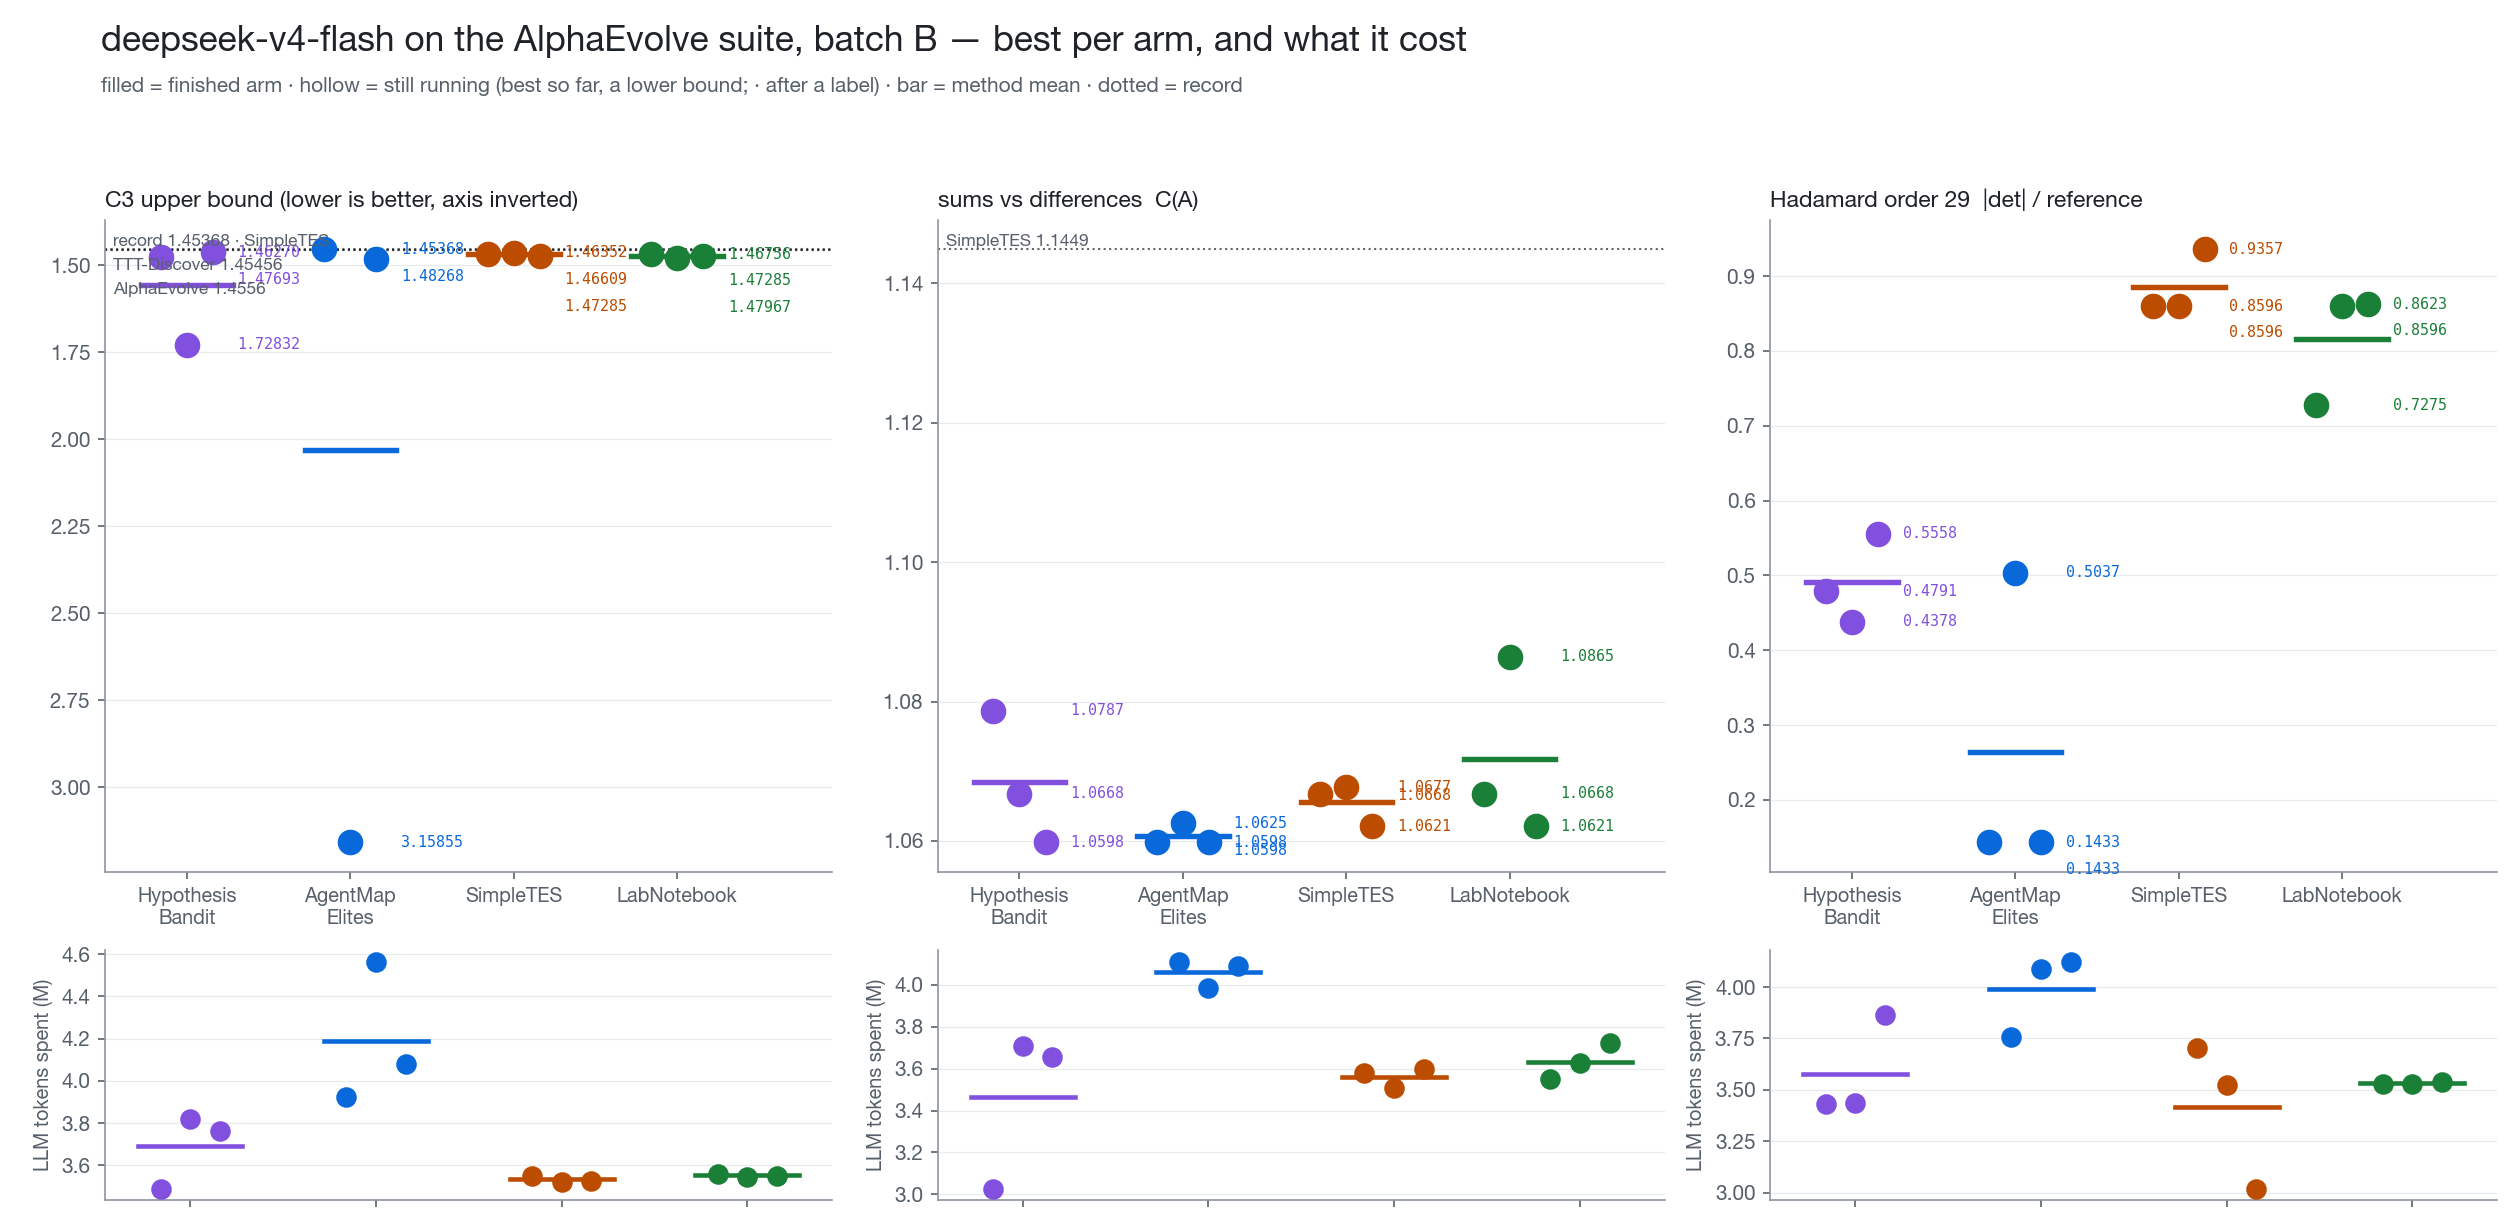
\includegraphics[width=\textwidth]{lab_notebook_figs/overview_ae_batchB.png}
\caption{Batch B, all arms finished. $C_3$ and Hadamard go to SimpleTES, sums vs differences to
LabNotebook; on $C_3$ the two are within replicate spread.}
\end{figure}

\paragraph{Batch C.} Three CodeEvolve-instance tasks --- kissing number in $d{=}11$, Heilbronn
triangle $n{=}11$, Heilbronn convex $n{=}13$ --- scored as the ratio of the construction's value to
AlphaEvolve's published one (1.0 = AlphaEvolve), with CodeEvolve's verifiers verbatim and their stub
seeds (a valid but empty construction). All 36 arms finished.

\begin{table}[H]\centering\small
\caption{Batch C, all 36 arms finished: ratio to AlphaEvolve per arm (higher is better).}
\label{tab:aec}
\begin{tabular}{@{}lrrrrr@{}}
\toprule
\multicolumn{6}{@{}l}{\textbf{kissing number, $d{=}11$}} \\
method & s0 & s1 & s2 & mean & tokens \\
\midrule
HypothesisBandit & 0.5868 & 0.6998 & 0.3710 & 0.5526 & 3.3 \\
AgentMapElites & 0.9174 & 0.0034 & 0.0034 & 0.3080 & 3.8 \\
\textbf{SimpleTES} & 0.9815 & 0.9815 & 0.9815 & \textbf{0.9815} & 3.2 \\
LabNotebook & 0.9680 & 0.9815 & 0.9815 & 0.9770 & 3.6 \\
\midrule
\multicolumn{6}{@{}l}{\textbf{Heilbronn triangle, $n{=}11$}} \\
\midrule
HypothesisBandit & 0.5986 & 0.2785 & 0.9180 & 0.5984 & 3.9 \\
AgentMapElites & 0.8822 & 0.8275 & 0.8882 & 0.8660 & 3.7 \\
SimpleTES & \textbf{0.9962} & 0.7543 & 0.9035 & 0.8847 & 1.7 \\
LabNotebook & 0.8382 & 0.9583 & 0.8648 & \textbf{0.8871} & 3.6 \\
\midrule
\multicolumn{6}{@{}l}{\textbf{Heilbronn convex, $n{=}13$}} \\
\midrule
HypothesisBandit & 0.6624 & 0.7561 & 0.8798 & 0.7661 & 3.8 \\
AgentMapElites & 0.7735 & 0.7928 & 0.8638 & 0.8100 & 3.9 \\
SimpleTES & 0.9158 & 0.8676 & 0.8833 & 0.8889 & 3.6 \\
\textbf{LabNotebook} & 0.8520 & \textbf{1.0000} & 0.8905 & \textbf{0.9142} & 3.6 \\
\bottomrule
\end{tabular}
\end{table}

\begin{figure}[H]\centering
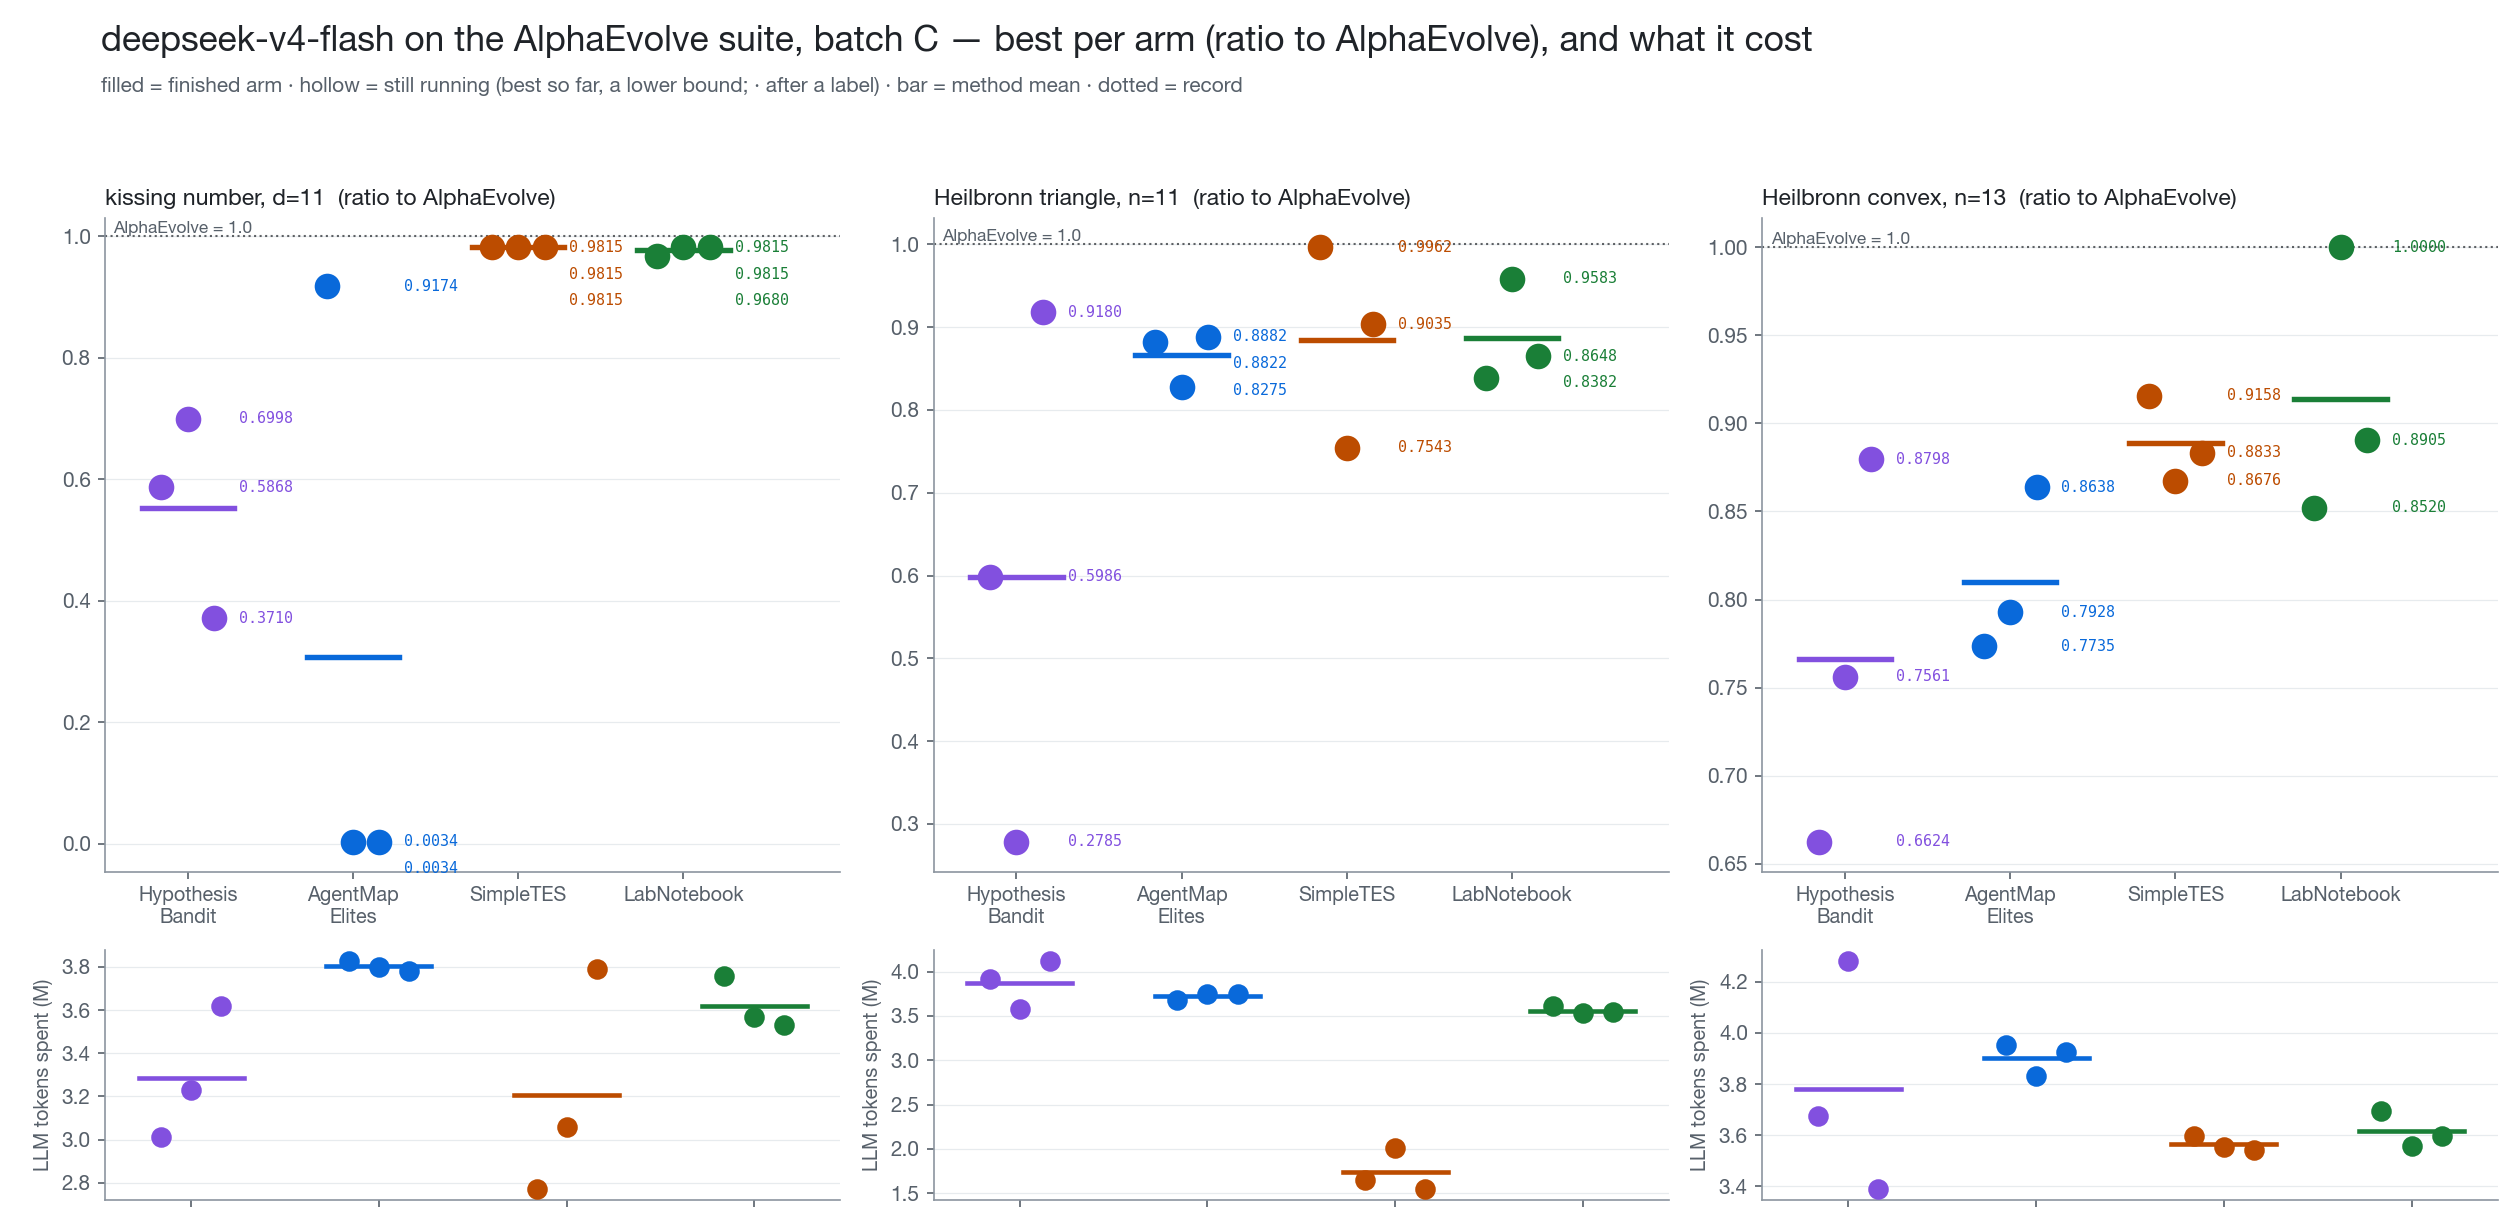
\includegraphics[width=\textwidth]{lab_notebook_figs/overview_ae_batchC.png}
\caption{Batch C. Kissing-11 and Heilbronn-triangle are ties within replicate spread (SimpleTES
reaches 0.9815 on every kissing arm, LabNotebook on two); Heilbronn-convex goes to LabNotebook,
whose s1 arm matches AlphaEvolve's value exactly.}
\end{figure}

\paragraph{Batch D.} The last three CodeEvolve-instance tasks --- min/max distance ratio
$n{=}16$, circles in a rectangle $n{=}21$, hexagons in a hexagon $n{=}11$ --- scored as the ratio to
AlphaEvolve's value. All 36 arms finished (one LabNotebook arm hung after a preemption resume and
was relaunched from its checkpoint). On hexagon-11 SimpleTES produced no program at all: the seed
is long, and all 24 of its whole-program completions ended without a closing code fence, so its
three arms report the seed value; MAP-Elites also never left the seed there and never found a
valid rectangle packing.

\begin{table}[H]\centering\small
\caption{Batch D, all 36 arms finished: ratio to AlphaEvolve per arm (higher is better).}
\label{tab:aed}
\begin{tabular}{@{}lrrrrr@{}}
\toprule
\multicolumn{6}{@{}l}{\textbf{min/max distance ratio, $n{=}16$}} \\
method & s0 & s1 & s2 & mean & tokens \\
\midrule
HypothesisBandit & 0.9991 & 0.9958 & 0.8821 & 0.9590 & 3.6 \\
AgentMapElites & 0.9957 & 0.9999 & 0.9915 & 0.9957 & 3.7 \\
\textbf{SimpleTES} & 1.0000 & 1.0000 & 1.0000 & \textbf{1.0000} & 3.5 \\
LabNotebook & 1.0000 & 0.9980 & 1.0000 & 0.9993 & 3.6 \\
\midrule
\multicolumn{6}{@{}l}{\textbf{circles in a rectangle, $n{=}21$}} \\
\midrule
HypothesisBandit & 0.9770 & 0.9949 & 1.0000 & 0.9906 & 3.7 \\
AgentMapElites & 0.0000 & 0.0000 & 0.0000 & 0.0000 & 3.8 \\
SimpleTES & 0.9979 & 0.9993 & 0.9869 & 0.9947 & 3.6 \\
\textbf{LabNotebook} & 1.0000 & 0.9974 & 1.0000 & \textbf{0.9991} & 3.5 \\
\midrule
\multicolumn{6}{@{}l}{\textbf{hexagons in a hexagon, $n{=}11$}} \\
\midrule
\textbf{HypothesisBandit} & 0.9066 & \textbf{0.9825} & 0.9818 & \textbf{0.9570} & 3.9 \\
AgentMapElites & 0.4913 & 0.4913 & 0.4913 & 0.4913 & 4.0 \\
SimpleTES & 0.4913$^\S$ & 0.4913$^\S$ & 0.4913$^\S$ & 0.4913 & 3.7 \\
LabNotebook & 0.9470 & 0.6271 & \textbf{0.9825} & 0.8522 & 3.6 \\
\multicolumn{6}{@{}l}{\footnotesize $^\S$ seed value: every completion came back without a code block} \\
\bottomrule
\end{tabular}
\end{table}

\begin{figure}[H]\centering
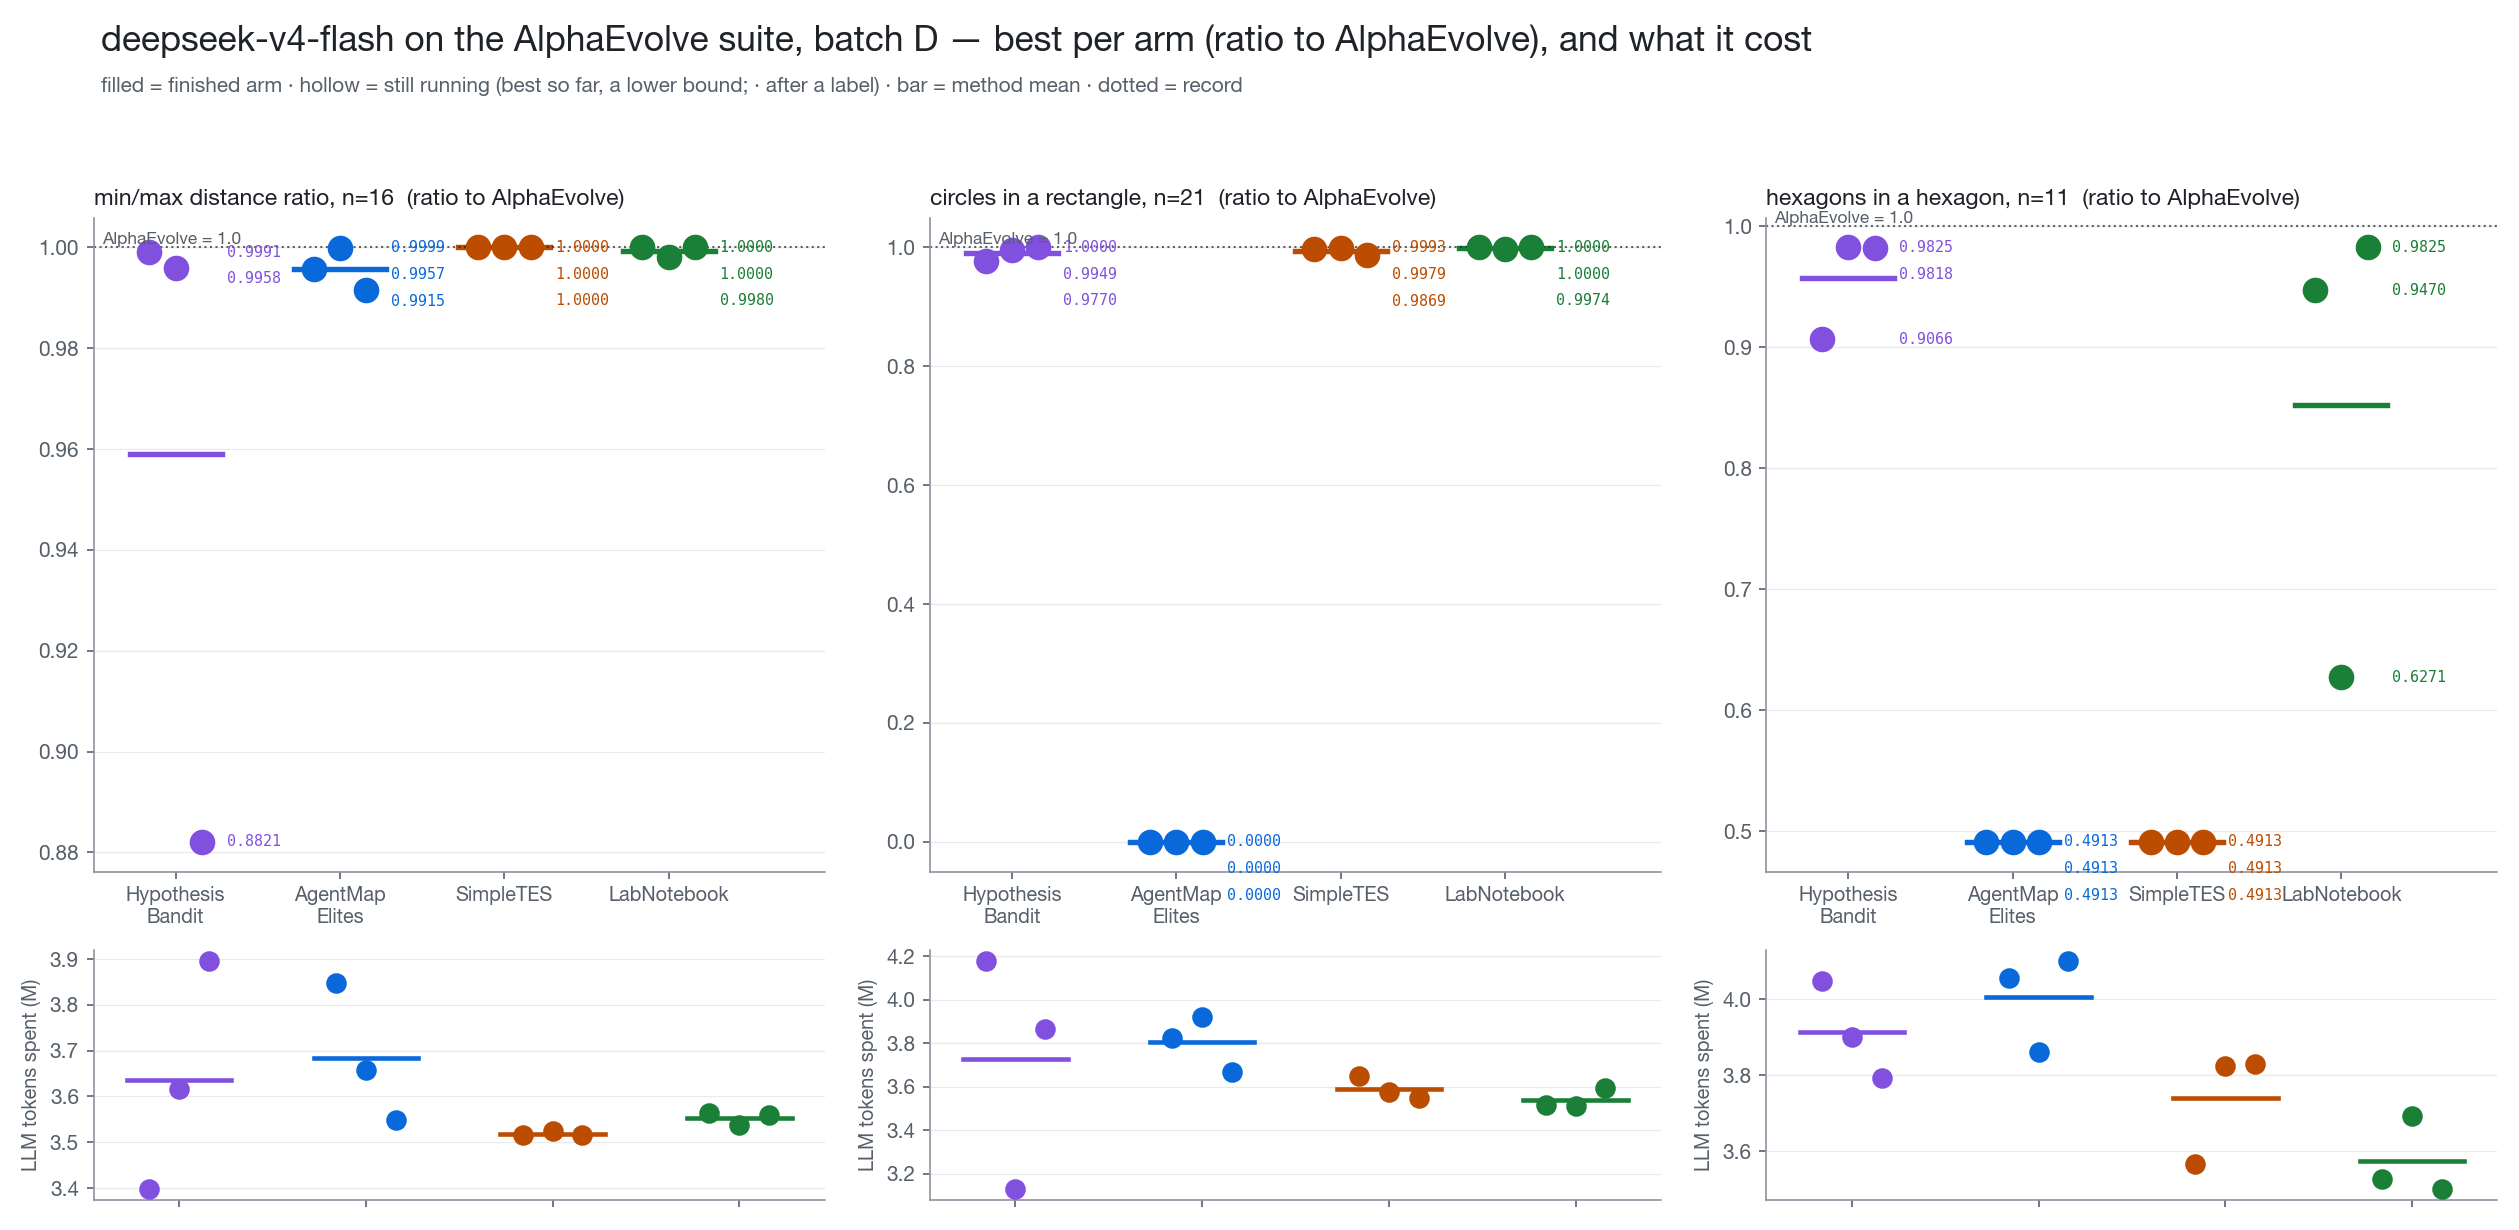
\includegraphics[width=\textwidth]{lab_notebook_figs/overview_ae_batchD.png}
\caption{Batch D. Min/max and rectangle packing are ties at AlphaEvolve's value; hexagon-11 is
HypothesisBandit's, with LabNotebook second and SimpleTES unable to produce a program.}
\end{figure}

\subsection{Cost}

\begin{center}\small
\begin{tabular}{@{}lrrrrrr@{}}
\toprule
& \multicolumn{3}{c}{flash} & \multicolumn{3}{c}{pro} \\
\cmidrule(lr){2-4}\cmidrule(lr){5-7}
\$ per finished arm (arms) & AHC039 & packing & Erd\H{o}s & AHC039 & packing & Erd\H{o}s \\
\midrule
HypothesisBandit & \$0.79{\scriptsize\,(3)} & \$0.17{\scriptsize\,(3)} & \$0.16{\scriptsize\,(3)} & \$10.17{\scriptsize\,(3)} & \$2.07{\scriptsize\,(3)} & \$2.35{\scriptsize\,(3)} \\
AgentMapElites & \$0.82{\scriptsize\,(3)} & \$0.19{\scriptsize\,(3)} & \$0.19{\scriptsize\,(3)} & \$11.61{\scriptsize\,(3)} & \$2.55{\scriptsize\,(3)} & \$2.41{\scriptsize\,(3)} \\
SimpleTES & \$1.80{\scriptsize\,(3)} & \$0.29{\scriptsize\,(3)} & \$0.32{\scriptsize\,(3)} & \$42.27{\scriptsize\,(3)} & \$5.42{\scriptsize\,(3)} & \$5.97{\scriptsize\,(3)} \\
LabNotebook & \$1.26{\scriptsize\,(3)} & \$0.29{\scriptsize\,(3)} & \$0.31{\scriptsize\,(3)} & \$25.41{\scriptsize\,(3)} & \$5.20{\scriptsize\,(3)} & \$5.89{\scriptsize\,(3)} \\
\bottomrule
\end{tabular}
\end{center}

\noindent Token-priced at OpenRouter's rates (flash \$0.05/\$0.10 per M prompt/completion; pro
\$0.66/\$1.98), all arms finished. LabNotebook is not cheaper than the others: on the small tasks all four methods
spend to the same token ceiling, and on AHC039 --- where nothing but the call cap binds ---
LabNotebook and SimpleTES are the two methods that keep spending to the end (SimpleTES's pro AHC039
figure also carries the tokens of its interrupted runs). The five notebook calls per cycle are a small share of
that; the cost is the $K\,T\,k=16$ operator completions per cycle. An earlier note in this document
called LabNotebook the cheapest method; that was read from partial arms and is withdrawn.

\subsection{Baseline fidelity and ablations (in progress)}
\label{sec:parts}

Two follow-up studies address the two objections to the comparison above: that our SimpleTES is
a port, and that nothing yet attributes LabNotebook's results to its design. Both run in the same
harness, on the same tasks and budgets as the main campaigns, with \texttt{deepseek-v4-flash}.

\subsubsection*{Part 1 --- is the port a fair SimpleTES?}

The original SimpleTES engine (github.com/wq-will/SimpleTES, pinned at commit \texttt{a19a54b})
is run unmodified through an adapter that gives it our task's seed program, objective and
evaluator, our model through the same gateway, and --- for AHC039 --- the same eval server as
every other arm. Its checkpoint is converted into our summary format, and every request's tokens
are booked through a hook the adapter installs in the engine's interpreter (rejected generations
included, which the engine's own checkpoint does not keep).

SimpleTES's search has five knobs, and the study runs the engine under two settings of them:

\begin{center}\small
\begin{tabular}{@{}>{\raggedright\arraybackslash}p{28mm}>{\raggedright\arraybackslash}p{24mm}>{\raggedright\arraybackslash}p{26mm}>{\raggedright\arraybackslash}p{58mm}@{}}
\toprule
knob & \emph{port-mirror} & \emph{authors' defaults} & what it does \\
\midrule
chains & 2 & 4 & independent lineages evolved side by side; each keeps its own incumbent \\
$k$ candidates & 2 & 4 & completions per prompt; the best of the $k$ is committed to the chain \\
inspirations & 2 & 5 & reference programs shown in the prompt beside the parent \\
selector & rpucg & balance & the policy that picks those references from the database (rpucg is the engine's UCB-style rule; balance is its default exploitation/exploration mix) \\
reflection & off & on & an extra model call that writes a short reflection on each batch-best program and feeds it into later prompts \\
\midrule
seed evaluation & \multicolumn{3}{>{\raggedright\arraybackslash}p{112mm}}{both: once (the engine's default is 16 repeats, max kept)} \\
candidates & \multicolumn{3}{>{\raggedright\arraybackslash}p{112mm}}{both: 100 (60 on C1), each one request in the engine's streaming mode} \\
tokens & \multicolumn{3}{>{\raggedright\arraybackslash}p{112mm}}{both: 64k output per request; 3.5\,M completion-token cap} \\
evaluation & \multicolumn{3}{>{\raggedright\arraybackslash}p{112mm}}{both: our evaluator, 300 s; AHC039 on the shared eval server} \\
\bottomrule
\end{tabular}
\end{center}

\emph{Port-mirror} is the configuration our port ran in the main campaigns (\S\ref{sec:flash}),
so an upstream arm in this setting differs from a port arm only in the code that implements the
search: it measures implementation fidelity. \emph{Authors' defaults} is the engine as shipped
--- wider (4 chains, $k{=}4$), more context (5 inspirations), its default selector, and the
reflection call our port deliberately omits: it measures whether the settings we chose for the
port handicapped SimpleTES. If the two upstream settings and the port all land within replicate
spread of each other, the comparison with LabNotebook stands as measured; if either upstream
setting is clearly stronger, the honest baseline becomes that setting.

Two accounting facts to keep in view when reading the tokens column: the engine's token cap counts
completion tokens only, so its arms consume more total tokens than our 3.5\,M cap on prompt
and completion together (3.1--6.7\,M on the finished arms); and the engine rejects a reply that drops the
\texttt{EVOLVE-BLOCK} markers or comes back empty --- with this model that is common (1--60
rejections per arm so far) and it counts against the candidate budget, as the authors' contract
intends.

\subsubsection*{Part 2 --- which parts of LabNotebook do the work?}

A full LabNotebook cycle makes these model calls: \call{Propose} ($K{=}4$ ideas), then $K \times
T = 8$ operator steps (each one request returning $k{=}2$ candidates; the idea rides in every
step's instruction), then $K = 4$ \call{Digest} calls and one \call{Update} of the notebook; the
notebook itself comes from one \call{Understand} call at the start. Each ablation removes
\emph{exactly one} of these and leaves everything else --- budgets, operator, parent selection,
references --- unchanged:

\begin{center}\small
\begin{tabular}{@{}>{\raggedright\arraybackslash}p{24mm}>{\raggedright\arraybackslash}p{46mm}>{\raggedright\arraybackslash}p{27mm}>{\raggedright\arraybackslash}p{44mm}@{}}
\toprule
variant & what changes & calls per cycle & what it tests \\
\midrule
full & --- & 1 + 8 + 4 + 1 & the reference \\
no ideas & \call{Propose} is skipped; the $K$ trajectories run with the plain objective as
  instruction (exactly what the port sends); digests and notebook still run & 0 + 8 + 4 + 1 &
  whether the gain comes from steering by explicit ideas, or merely from the parallel-short-trajectory
  structure \\
one long trajectory & $K{=}1$, $T{=}8$: one idea, one trajectory of eight chained steps, still
  16 candidates per cycle; fewer outer calls, so $\sim$40\% more cycles per budget & 1 + 8 + 1 + 1 &
  breadth (four shallow probes) against depth (one deep pursuit) --- the trajectory-length hypothesis \\
no notebook & \call{Understand} and \call{Update} are skipped; \call{Propose} sees the problem, the
  history table (numbers and digests) and the parent program, but no accumulated prose understanding &
  1 + 8 + 4 + 0 & whether the rewritten understanding improves idea quality beyond the raw record \\
no digest & \call{Digest} is skipped; history rows keep the numbers (idea, predicted and measured
  gain, candidates) but no outcome/why/lesson; the notebook update sees numbers only & 1 + 8 + 0 + 1 &
  whether the model's written interpretation of each experiment matters, or the numbers suffice \\
\bottomrule
\end{tabular}
\end{center}

The inner step of every variant is SimpleTES's operator; the table below lists its knobs as run,
beside the port and the authors' engine. Note that the selector, though nominally different, never
chooses in LabNotebook: a trajectory of $T{=}2$ steps holds at most the parent and one committed
child, and with two inspirations requested the selector returns the whole chain. So the inner steps
are plain SimpleTES steps; what LabNotebook changes is the chains' length and count ($4 \times 2$,
restarted from a chosen parent, against two long chains), the idea injected into the instruction,
and the parent choice between cycles.

\begin{center}\small
\begin{tabular}{@{}>{\raggedright\arraybackslash}p{30mm}>{\raggedright\arraybackslash}p{50mm}>{\raggedright\arraybackslash}p{30mm}>{\raggedright\arraybackslash}p{30mm}@{}}
\toprule
knob & LabNotebook inner loop & our port (bench) & upstream, port-mirror \\
\midrule
operator / prompt & SimpleTES's completion prompt verbatim, with the idea block appended & same prompt, no idea & the engine's own \\
candidates per step ($k$) & 2: one request with $n{=}2$, best of two committed & 2 & 2 \\
inspirations per step & 2, from the trajectory's own chain & 2, from the chain & 2 \\
chains & $K{=}4$ trajectories per cycle, each restarted from the cycle's parent, $T{=}2$ steps & 2, continuous & 2 \\
selector & balance (never invoked at $T{=}2$, see text) & rpucg & rpucg \\
output cap / temperature / reflection & 64k tokens, 1.0, none & same & same \\
parent of a new chain & champion w.p.\ 0.7, else a reference from another idea lineage & its own chain head & its own chain head \\
\bottomrule
\end{tabular}
\end{center}

Two further variants are implemented but not yet run: \emph{generic ideas} (a fixed list sampled
per cycle, no model call --- diversity without judgement) and $k$-vs-$T$ trade-offs.

The ablations run on the two cheap tasks where LabNotebook led (C2, sums vs differences) and on
AHC039, where the effect to explain is largest (40 points in the pro campaign). On AHC039 all
variants run as one block of three waves, each wave one seed with every method --- the authors'
engine, a fresh LabNotebook, a fresh port, and the four ablations --- on its own eval server, so
within a wave every method sees the same machine and load, and the waves are blocked replicates;
warm-up evaluation and a 20-minute seed drift probe calibrate the three servers. Reading rule: a
variant's effect is its difference from the full method on the same task; on the cheap tasks
differences inside the replicate spread ($\sim$0.01) are inconclusive, on AHC039 the bar is
$\sim$20 points, the seed's own machine noise.

\begin{table}[H]\centering\small
\caption{Part 1, all 21 upstream-engine arms finished (2026-09-10 01:05 PDT): best per arm (s0 / s1 / s2)
and mean.}
\label{tab:part1}
\begin{tabular}{@{}lrrrr@{}}
\toprule
\multicolumn{5}{@{}l}{\textbf{$C_2$} (higher is better)} \\
group & s0 & s1 & s2 & mean \\
\midrule
LabNotebook & 0.9248 & 0.9106 & 0.9185 & 0.9180 \\
our SimpleTES port & 0.9101 & 0.9079 & 0.9139 & 0.9106 \\
upstream, port-mirror & 0.9112 & 0.9133 & 0.9269 & 0.9172 \\
upstream, authors' defaults & 0.9120 & 0.9094 & 0.9093 & 0.9102 \\
\midrule
\multicolumn{5}{@{}l}{\textbf{sums vs differences} (higher is better)} \\
\midrule
LabNotebook & 1.0668 & 1.0865 & 1.0621 & 1.0718 \\
our SimpleTES port & 1.0668 & 1.0677 & 1.0621 & 1.0655 \\
upstream, port-mirror & 1.0692 & 1.0865 & 1.0759 & 1.0772 \\
upstream, authors' defaults & 1.0668 & 1.0668 & 1.0668 & 1.0668 \\
\midrule
\multicolumn{5}{@{}l}{\textbf{Heilbronn convex $n{=}13$} (ratio, higher is better)} \\
\midrule
LabNotebook & 0.8520 & 1.0000 & 0.8905 & 0.9142 \\
our SimpleTES port & 0.9158 & 0.8676 & 0.8833 & 0.8889 \\
upstream, port-mirror & 0.8614 & 0.8877 & 0.9163 & 0.8884 \\
upstream, authors' defaults & 0.7127 & 0.8554 & 0.7126 & 0.7602 \\
\midrule
\multicolumn{5}{@{}l}{\textbf{$C_1$ control} (lower is better)} \\
\midrule
LabNotebook & 1.51063 & 1.51267 & 1.50947 & 1.51093 \\
our SimpleTES port & 1.50941 & 1.51148 & 1.51088 & 1.51059 \\
upstream, port-mirror & 1.51467 & 1.51120 & 1.50894 & 1.51160 \\
\bottomrule
\end{tabular}
\end{table}

\begin{figure}[H]\centering
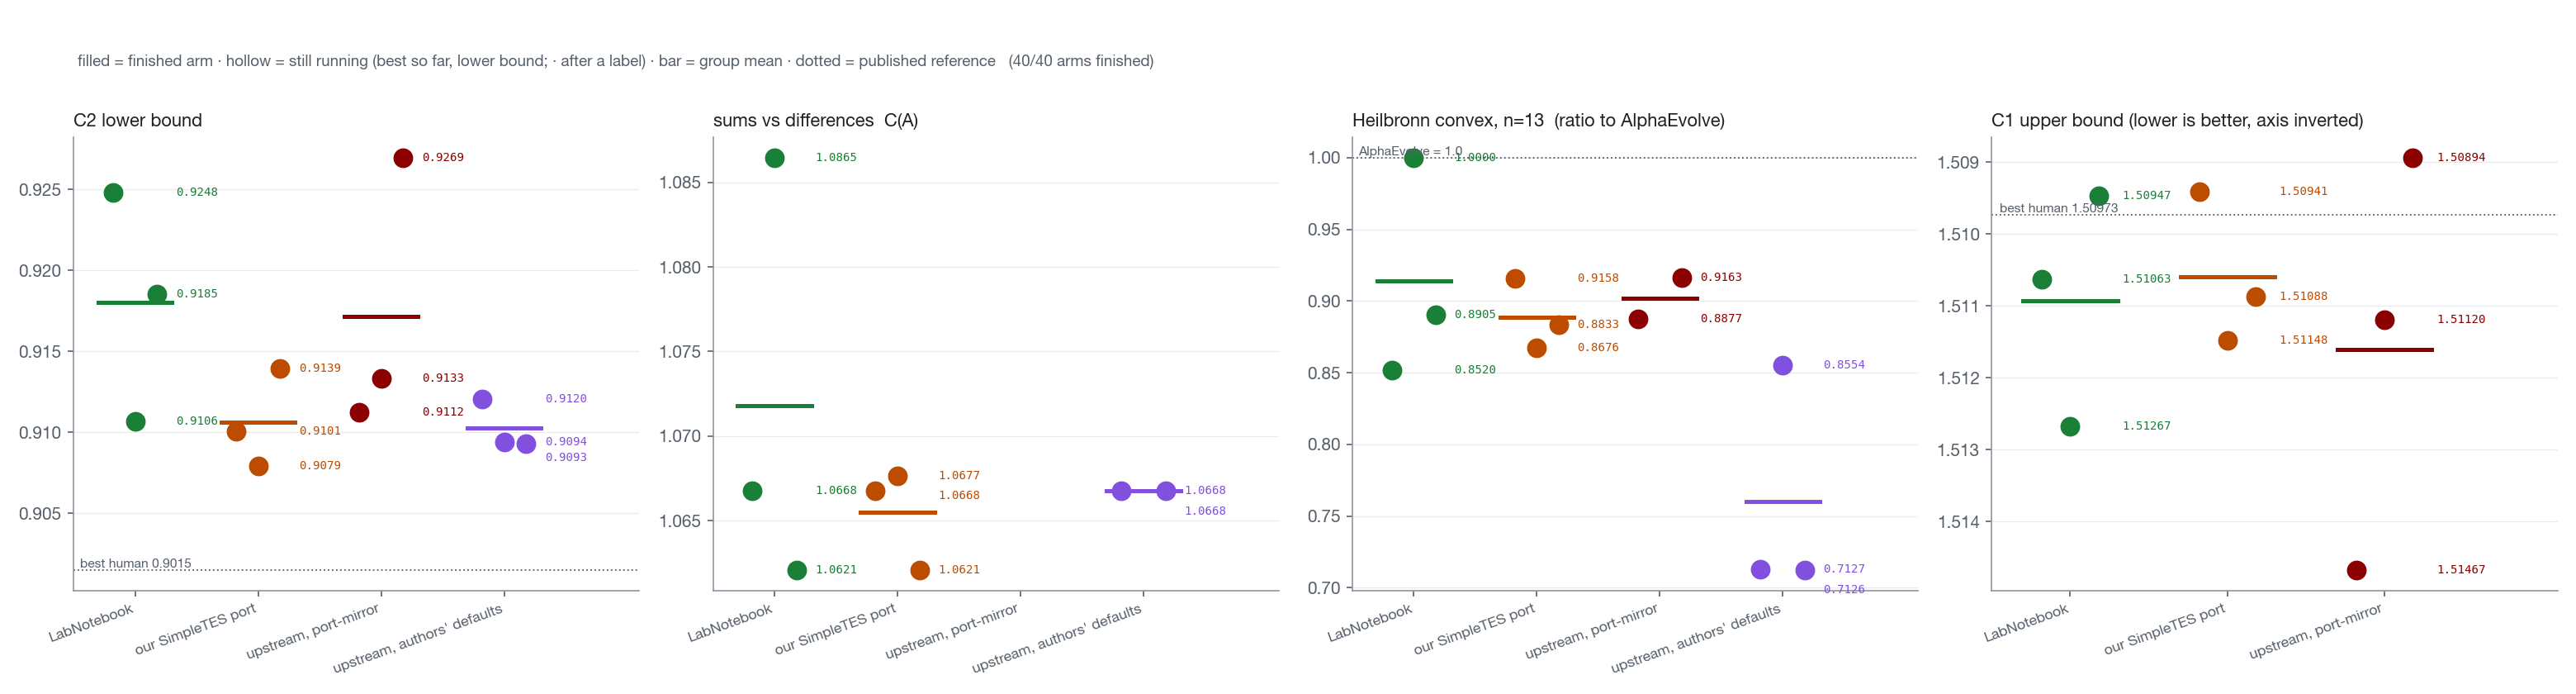
\includegraphics[width=\textwidth]{lab_notebook_figs/part1_upstream_vs_port.png}
\caption{Part 1, final. The authors' engine lands inside our port's replicate range on every task
under the port-mirror knobs, and above it on sums vs differences (mean 1.0772 against the port's
1.0655 and LabNotebook's 1.0718). Under the authors' own defaults it is at or below the port
everywhere. Nothing here indicates the port is a weaker baseline than the original; on sums vs
differences the mirror is, if anything, the stronger SimpleTES.}
\end{figure}

\begin{table}[H]\centering\small
\caption{Part 2: the AHC039 ablation block (official points, best per arm, s0 / s1 / s2 and mean). All 21
arms finished on Sherlock under one configuration: deepseek-v4.1-flash without thinking, 32k output
limit, block-edit-only merge, three retries, one eval server per wave, equal 480-call budgets. Seed
re-reads during the block sat at 3686--3711 points, so differences below $\sim$20 points are machine
noise.}
\label{tab:part2}
\begin{tabular}{@{}lrrrr@{}}
\toprule
method & s0 & s1 & s2 & mean \\
\midrule
LabNotebook (full) & \textbf{3787} & 3728 & 3749 & \textbf{3755} \\
no ideas & 3717 & 3707 & 3718 & 3714 \\
one long trajectory & 3718 & 3712 & 3735 & 3722 \\
no notebook & 3731 & 3740 & 3714 & 3728 \\
no digest & 3717 & 3726 & 3725 & 3723 \\
\midrule
our SimpleTES port & 3691 & 3721 & 3734 & 3715 \\
upstream SimpleTES & 3711 & 3698 & 3652 & 3687 \\
\bottomrule
\end{tabular}
\end{table}

\begin{figure}[H]\centering
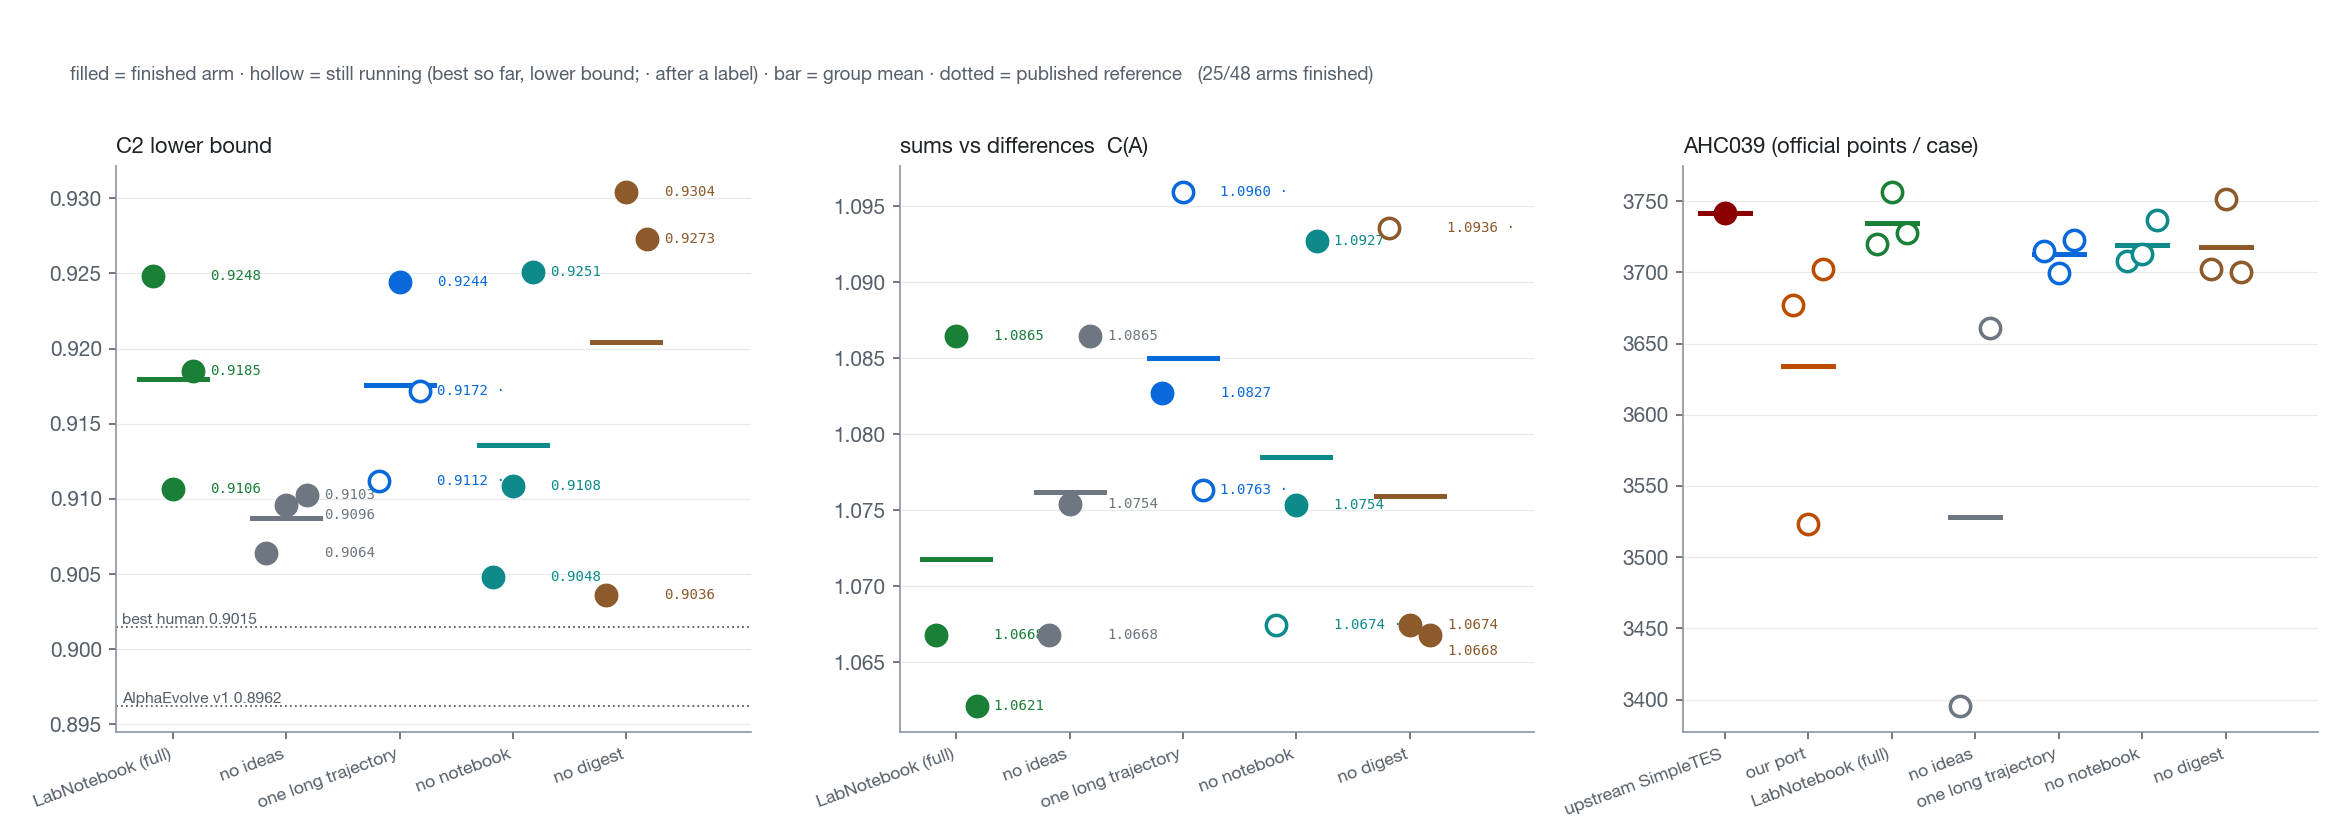
\includegraphics[width=\textwidth]{lab_notebook_figs/part2_ablations.png}
\caption{Part 2, the AHC039 ablation block. The full method leads at 3755 points with every seed at or
above 3728; removing the ideas drops to 3714, the level of our SimpleTES port (3715), so the ideas
carry the effect; removing the notebook (3728) or the digest (3723), or running one long trajectory
(3722), each cost about 30 points, at the edge of the $\sim$20-point noise band. The two SimpleTES
versions (our port and the authors' engine, 3687) are the rightmost columns.}
\end{figure}

\paragraph{The same ablations on the other tasks where LabNotebook leads.} Hexagon-11
and Heilbronn convex-13 are the two AlphaEvolve-suite tasks on which LabNotebook led the port
(Table~\ref{tab:h2h}). The four ablations were run there (three seeds each, AlphaEvolve-suite budgets,
deepseek-v4-flash-0731); the full-method and port references are the AlphaEvolve-campaign arms
themselves. Table~\ref{tab:ablc} and Figure~\ref{fig:ablc} carry the results.

\begin{table}[H]\centering\small
\caption{Ablations on hexagon-11 and Heilbronn convex-13, all 30 arms finished (three seeds each, AlphaEvolve-suite budgets, deepseek-v4-flash-0731). Best per arm (s0 / s1 / s2) and mean; higher is better. The full-method and port rows are the AlphaEvolve-campaign arms. \emph{no memory} = ideas proposed from the problem and the parent program alone: no notebook, no digest, and the record of tried ideas hidden from the proposer (\texttt{--ln-no-notebook --ln-no-digest --ln-no-history}).}
\label{tab:ablc}
\begin{tabular}{@{}lrrrr@{}}
\toprule
\multicolumn{5}{@{}l}{\textbf{hexagon 11} (ratio to the published value)} \\
method & s0 & s1 & s2 & mean \\
\midrule
LabNotebook (full) & 0.9470 & 0.6271 & 0.9825 & 0.8522 \\
no ideas & 0.7860 & 0.4913 & 0.7706 & 0.6826 \\
one long trajectory & 0.9774 & 0.4913 & 0.9820 & 0.8169 \\
no notebook & 0.8804 & 0.9823 & 0.9711 & 0.9446 \\
no digest & 0.9825 & 0.9825 & 0.9825 & 0.9825 \\
no memory & 0.6966 & 0.4913 & 0.9576 & 0.7152 \\
\midrule
our SimpleTES port & 0.4913 & 0.4913 & 0.4913 & 0.4913 \\
\midrule
\multicolumn{5}{@{}l}{\textbf{Heilbronn convex $n{=}13$} (ratio, higher is better)} \\
\midrule
LabNotebook (full) & 0.8520 & 1.0000 & 0.8905 & 0.9142 \\
no ideas & 0.7344 & 0.5696 & 0.6876 & 0.6639 \\
one long trajectory & 0.9211 & 0.7663 & 0.8285 & 0.8386 \\
no notebook & 0.9296 & 0.9218 & 0.8657 & 0.9057 \\
no digest & 0.8420 & 0.8621 & 0.9296 & 0.8779 \\
no memory & 0.9293 & 0.9911 & 0.9086 & \textbf{0.9430} \\
\midrule
our SimpleTES port & 0.9158 & 0.8676 & 0.8833 & 0.8889 \\
\bottomrule
\end{tabular}
\end{table}

\begin{figure}[H]\centering
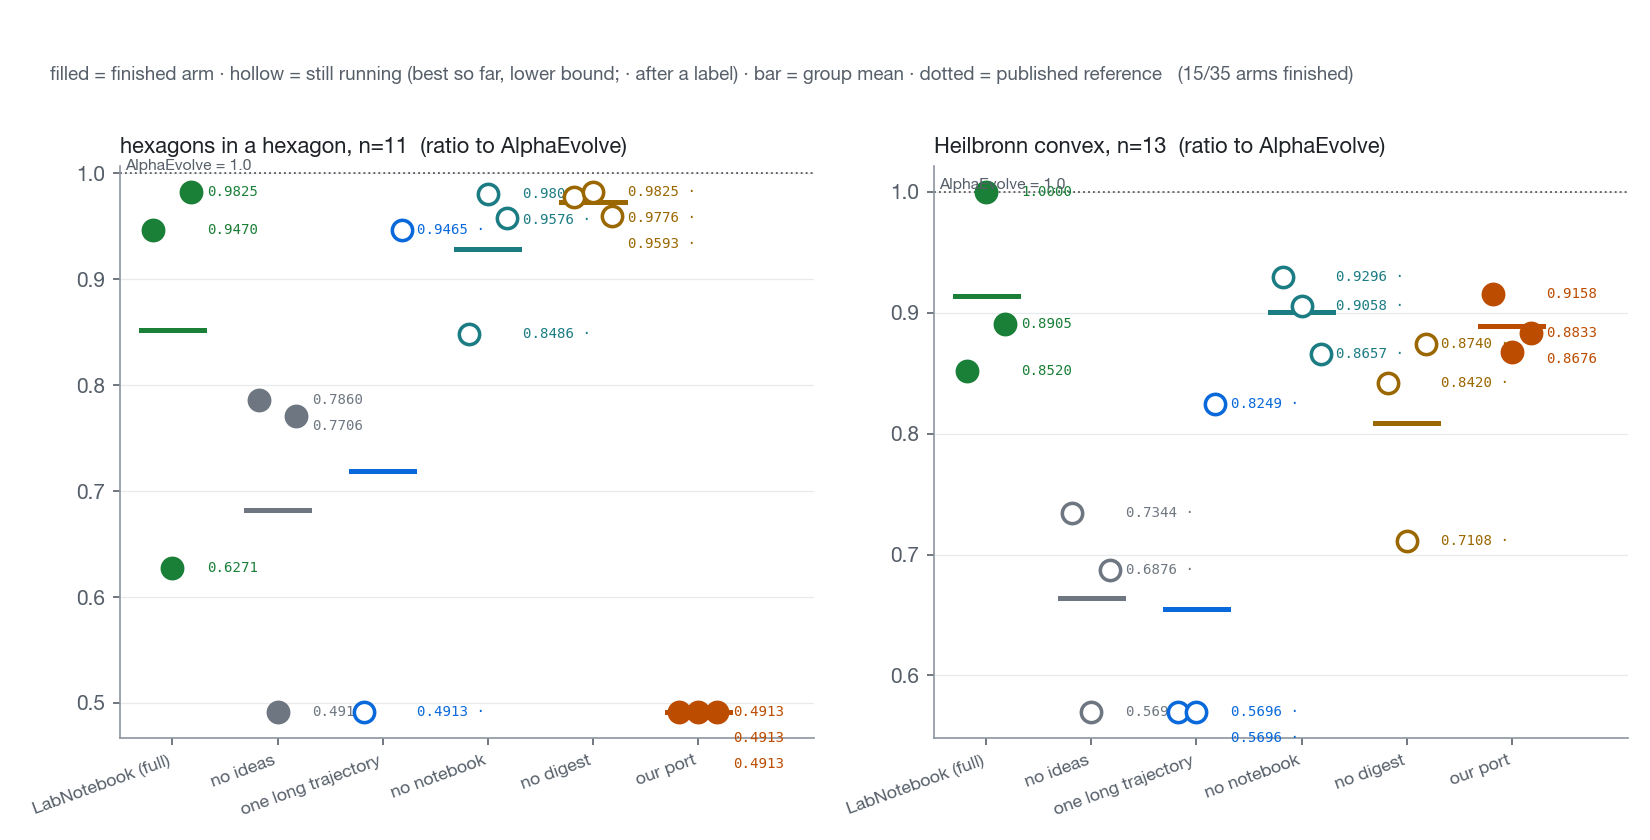
\includegraphics[width=\textwidth]{lab_notebook_figs/partC_ablations.png}
\caption{Ablations on hexagon-11 (left) and Heilbronn convex-13 (right), final. The pattern of the other
tasks repeats. Removing the ideas is the one change that hurts on both: hexagon-11 falls from 0.852
to 0.683 (one seed exactly at the port's 0.491), Heilbronn from 0.914 to 0.664, below even the port
(0.889). Removing the notebook or the digest does not hurt and on hexagon-11 helps: no-digest
reaches the published value (0.9825) on all three seeds, no-notebook 0.945, against 0.852 for the
full method whose seed 1 stalled at 0.627. One long trajectory is the high-variance variant: on
hexagon-11 two seeds reach 0.98 and the third finds only the port-level packing (0.491); on Heilbronn
its mean (0.839) is below the full method and the port. The no-memory arm (added later, rightmost of
the LabNotebook groups) is the best group on Heilbronn (0.943, all three seeds above the port) and
sits between no-ideas and the full method on hexagon-11 (0.715, one seed at the port-level packing,
one at 0.958).}
\label{fig:ablc}
\end{figure}



\paragraph{Three more AHC tasks: AHC058, AHC046 and AHC026.} To test whether the AHC039
pattern (Table~\ref{tab:part2}) holds on other AtCoder heuristic contests, the same 21-arm block
(same configuration, budgets and one eval server per task) was run on Sherlock on AHC058 (Apple
Incremental Game), AHC046 (Skating with Blocks) and AHC026 (Stack of Boxes), all from ALE-Bench with
their official generators and scorers, 150 public cases each. Table~\ref{tab:abld} and
Figure~\ref{fig:abld} carry the results. The AHC039 pattern does not repeat on any of the three. On
AHC058 our SimpleTES port has the best mean (5.327) with all three seeds above 5.28, while the full
method has one weak seed (5.159) next to the single best arm of the block (5.371); on AHC046 the
no-ideas variant leads (1.451, three seeds within 0.006) with the full method second (1.430); on
AHC026 the port (0.926), the no-ideas variant (0.926) and the authors' engine (0.926) tie at the top
and the full method (0.918, seeds 0.915--0.921) is below every port seed (0.924--0.927), the one
clear loss among the AHC blocks. The spread of the seven method means is 1.4\% on AHC058, 2.3\% on
AHC046 and 1.0\% on AHC026, while one method's three seeds span 4\% (LabNotebook on AHC058) to 6\%
(the port on AHC046): except for AHC026, three seeds cannot separate any two methods on these tasks.
Two things do survive the noise. First, the items column: under the shared 480-call budget the full
method evaluates about a quarter fewer candidates than the port (175 against 238 on AHC058, 181
against 290 on AHC046, 174 against 226 on AHC026), because its Understand, Propose, Digest and
Update calls are booked against the same budget. On these incremental-tuning tasks, where the seed
heuristic is already strong and the gains come from many small local edits, the number of
evaluated edits matters more than their diversity. Second, no ablation moves the score by more than
the seed noise: on these three tasks neither the ideas nor the notebook nor the digest has a
measurable effect, and the variant that drops the ideas is never worse than the full method.

\begin{table}[H]\centering\small
\caption{The AHC039 block repeated on AHC058, AHC046 and AHC026, all 63 arms finished (three seeds
each, deepseek-v4.1-flash without thinking, 480-call budgets, best per arm and mean, higher is
better). \emph{items} = mean number of candidates the arm evaluated within the budget. Seed programs
re-read at 4.8675 (AHC058), 1.1266 (AHC046) and 0.8565 (AHC026) on every server.}
\label{tab:abld}
\begin{tabular}{@{}lrrrrr@{}}
\toprule
\multicolumn{6}{@{}l}{\textbf{AHC058} (official points, millions)} \\
method & s0 & s1 & s2 & mean & items \\
\midrule
LabNotebook (full) & 5.3246 & 5.1586 & \textbf{5.3710} & 5.2847 & 175 \\
no ideas & 5.2584 & 5.2784 & 5.2475 & 5.2614 & 183 \\
one long trajectory & 5.3215 & 5.2631 & 5.2851 & 5.2899 & 213 \\
no notebook & 5.3183 & 5.2549 & 5.2427 & 5.2720 & 182 \\
no digest & 5.2334 & 5.3191 & 5.2109 & 5.2545 & 212 \\
\midrule
our SimpleTES port & 5.3338 & 5.3642 & 5.2840 & \textbf{5.3274} & 238 \\
upstream SimpleTES & 5.2657 & 5.2574 & 5.2482 & 5.2571 & 480 \\
\midrule
\multicolumn{6}{@{}l}{\textbf{AHC046} (official points, thousands)} \\
\midrule
LabNotebook (full) & 1.4510 & 1.4437 & 1.3963 & 1.4303 & 181 \\
no ideas & 1.4479 & \textbf{1.4530} & 1.4533 & \textbf{1.4514} & 184 \\
one long trajectory & 1.4530 & 1.3791 & 1.4246 & 1.4189 & 253 \\
no notebook & 1.4431 & 1.4502 & 1.3612 & 1.4182 & 183 \\
no digest & 1.4097 & 1.4022 & 1.4436 & 1.4185 & 213 \\
\midrule
our SimpleTES port & 1.3611 & 1.4474 & 1.4494 & 1.4193 & 290 \\
upstream SimpleTES & 1.4170 & 1.4056 & 1.4404 & 1.4210 & 448 \\
\midrule
\multicolumn{6}{@{}l}{\textbf{AHC026} (official points / 10,000)} \\
\midrule
LabNotebook (full) & 0.9207 & 0.9184 & 0.9146 & 0.9179 & 174 \\
no ideas & 0.9211 & 0.9226 & \textbf{0.9334} & 0.9257 & 180 \\
one long trajectory & 0.9187 & 0.9280 & 0.9197 & 0.9221 & 194 \\
no notebook & 0.9284 & 0.9020 & 0.9185 & 0.9163 & 182 \\
no digest & 0.9232 & 0.9239 & 0.9174 & 0.9215 & 208 \\
\midrule
our SimpleTES port & 0.9262 & 0.9242 & 0.9269 & \textbf{0.9258} & 226 \\
upstream SimpleTES & 0.9200 & 0.9282 & 0.9290 & 0.9257 & 469 \\
\bottomrule
\end{tabular}
\end{table}

\begin{figure}[H]\centering
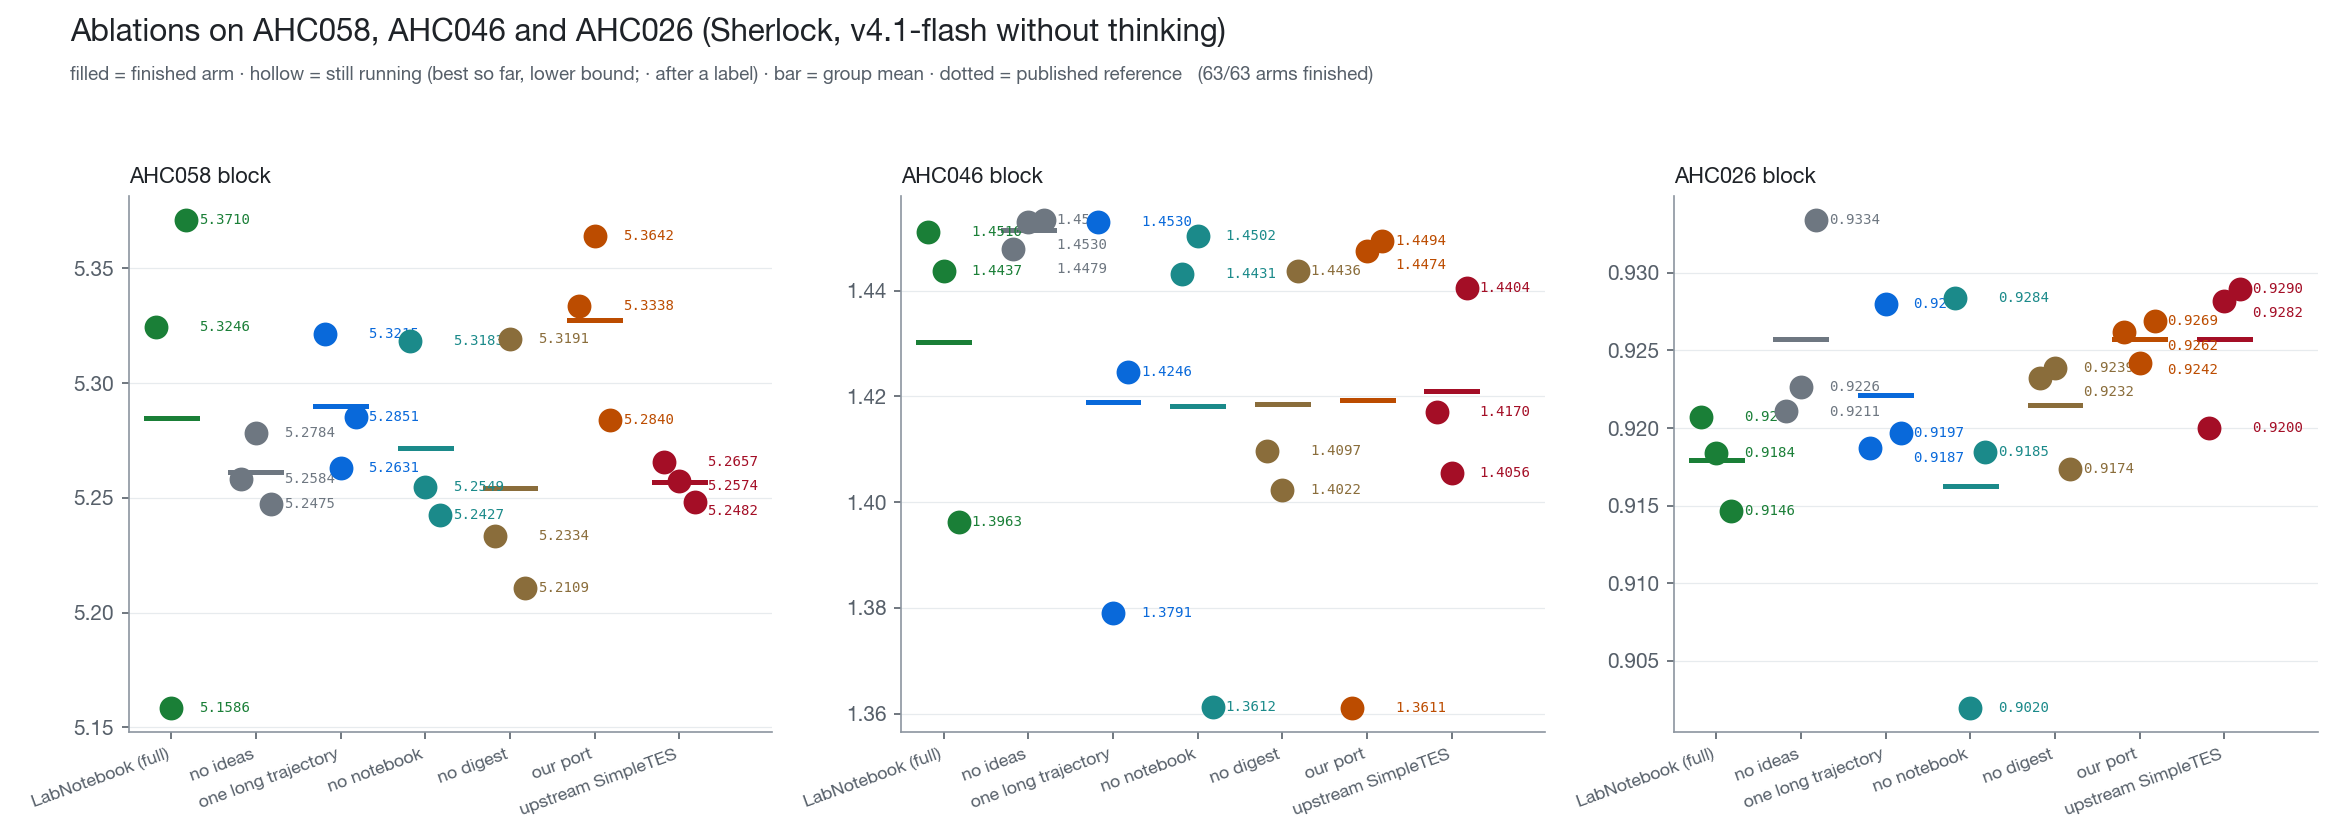
\includegraphics[width=\textwidth]{lab_notebook_figs/partD_ablations.png}
\caption{The ablation block on AHC058 (left), AHC046 (middle) and AHC026 (right), final. Unlike
AHC039 (Table~\ref{tab:part2}) and the two geometry tasks (Figure~\ref{fig:ablc}), no LabNotebook
variant separates from the others: the port leads AHC058 on the mean, the no-ideas variant leads
AHC046, the port, no-ideas and the authors' engine tie on AHC026, and on the first two every
group's three seeds overlap every other group's. On AHC026 the full method's three seeds
(0.915--0.921) all sit below the port's (0.924--0.927). The full method's AHC058 seed 1 (5.159) is
the lowest arm of that block and its seed 2 (5.371) the highest.}
\label{fig:abld}
\end{figure}

\paragraph{What the ablations remove, and what they do not.} Across the six tasks with a full
ablation block (AHC039, hexagon-11, Heilbronn-13, AHC058, AHC046, AHC026) the only two changes with effects
beyond seed noise are removing the ideas (hexagon-11 $-$20\%, Heilbronn-13 $-$27\%, AHC039 $-$1\%) and
collapsing the parallel short trajectories into one long one (Heilbronn-13 $-$8\%, hexagon-11 $-$4\%);
both are null on AHC058, AHC046 and AHC026. Removing the notebook or the digest is within noise on five tasks
and \emph{helps} on hexagon-11. One caveat on what these two switches test: \texttt{--ln-no-notebook}
drops only the prose notebook (the Understand and Update calls); the Propose call still sees the
full record of tried ideas with their numbers and, unless the digest is also off, the digest's
outcome and lesson for each. So the notebook ablation asks whether a 700-word prose summary adds
anything on top of the structured record, not whether memory matters. The arm that answers the
second question (ideas proposed from the problem and the parent program alone,
\texttt{--ln-no-history} with both other switches off) was run on hexagon-11 and Heilbronn-13, three
seeds each, and is the \emph{no memory} row of Table~\ref{tab:ablc}. Removing all memory costs
nothing: on Heilbronn-13 it is the best group of the block (0.943, every seed above the port's
0.889, against 0.914 for the full method), and on hexagon-11 it lands at 0.715, inside the full
method's own seed spread (0.627--0.983), with one seed at the port-level packing (0.491) and one at
0.958. Put next to no-ideas (0.683 and 0.664), the attribution is clean: what carries the effect on
these tasks is proposing ideas at all, fresh from the parent program each cycle, and running them
as parallel short trajectories; remembering which ideas were tried, digesting them, and keeping the
notebook add nothing measurable at this budget, while costing 5 of every 14 calls per cycle. The
most economical LabNotebook is therefore the no-memory one: one Propose call plus the trajectories.

\paragraph{Compute move (2026-09-09).} The Modal credit ran out on the morning of 2026-09-09. Every
arm still running there was cancelled at about 07:35 PDT and moved to Stanford's Sherlock cluster,
where it resumes from its last checkpoint (the bench checkpoints every two items, the upstream engine
every five evaluations; at most that much work was repeated). Moved: the whole selector study (24
arms, moved the evening before), the six unfinished ablation arms, the five unfinished Part 1 engine
arms, and the twenty unfinished AHC039 arms. Scores on the Python-evaluated tasks are machine
independent, so those arms continue unchanged. AHC039 is wall-clock limited: its arms will resume on
a Sherlock eval server, which is a different ruler from the Modal one, and the 20-minute seed probes
on both sides of the seam plus the server boot ids in every arm's log make the seam visible in the
analysis rather than averaged over. Finished arms are unaffected.

\paragraph{AHC039 block re-run, and a block-merge fix.} Because AHC039 scores are wall-clock limited, the
moved arms were not resumed: the whole block (21 arms, three waves, one eval server per wave, all
three servers on one Sherlock node) was restarted from scratch, and the Modal half-block is kept as a
separate dataset. Inspecting that half-block exposed a defect in our EVOLVE-BLOCK merge: a reply that
carried the whole file was spliced between the fixed prefix and suffix (declaring everything twice),
and a fence line nested inside the block survived into the source. Only 22\% of the half-block's
evaluations were compilable programs; 47\% were these two shapes. Every method using our variator
paid the same tax (the upstream engine rejects such replies outright), so the earlier AHC039
comparisons stand, but they were run at a quarter of the useful budget. The merge now finds the
innermost marker pair on fence-less text, takes a body that opens with a preprocessor line, defines
\texttt{main()}, or repeats the prefix as the whole program, and rejects a body with no statement
at all (prose, a formula, code in another language) so the variator re-rolls it. Checked against
213 real failures from a first, partial version of the fix, this keeps 147 whole programs whole and
rejects 14 junk replies; the expected share of compilable candidates rises from about a fifth to
about a half. The Sherlock block runs on this merge, and its AHC039 numbers are therefore not
comparable one-to-one with the flash/pro campaign's, which ran on the old merge.

\label{sec:merge}
\paragraph{What starved the port and no-ideas arms, and the final configuration.} The refined merge
had a second defect (it took the last marker pair in the reply; corrected), but that is not what
starved the arms. Captured replies were empty: every AHC039 spec had omitted
\texttt{--max-output-tokens}, so our methods ran at a 32\,768-token default while the engine arms in
the same specs ran at 64\,000, and DeepSeek-0731 thinks for 15--60k tokens on this task before it
writes, most of all on prompts without an idea to anchor on. Raising the limit did not help: at
64\,000 tokens a third of replies became from-scratch rewrites and long-reasoning replies compiled
only 8\% of the time; bounding the reasoning to 16k restored the item rate but 75\% of compilable
candidates were junk; and which OpenRouter host served a call set how long the model thought
(Makora and Inceptron 4--17k tokens and near-seed edits; six other hosts 26--63k, cut off or poor).
A controlled comparison at arm scale (no-ideas and port, the worst cases, $\sim$5 h each) settled it:
deepseek-v4.1-flash \emph{without} thinking produced 146 candidates, 95 compilable, 53 near the seed,
in the time every 0731 thinking configuration (32k, 64k, 100k) produced under ten. The final block
therefore runs deepseek-v4.1-flash with thinking disabled, a 32\,768-token limit, the block-edit-only
merge (whole-file replies and marker-carrying bodies rejected, as the upstream engine does), three
fresh rolls per empty reply, and the same settings injected into the upstream engine's calls. Its
AHC039 numbers are not comparable one-to-one with the flash/pro campaign's (0731 with thinking, old
merge); within the block every arm shares the configuration, and the earlier Modal half-block is
kept for provenance.

\paragraph{Trajectory length and the inspiration selector.} Because the selector never chooses at
$T{=}2$, a selector study has to lengthen the trajectories. Three arms per cell: $K{=}2$, $T{=}4$
(still 16 candidates per cycle) with balance and with rpucg; $K{=}1$, $T{=}8$ with rpucg (its
balance twin is the one-long ablation); and the port itself with balance (its rpucg twin is the
main-campaign port). Table~\ref{tab:sel} and Figure~\ref{fig:sel} carry the results.

\begin{table}[H]\centering\small
\caption{Selector study (2026-09-09 23:35 PDT), all 24 arms finished.}
\label{tab:sel}
\begin{tabular}{@{}lrrrr@{}}
\toprule
\multicolumn{5}{@{}l}{\textbf{$C_2$} (higher is better)} \\
group & s0 & s1 & s2 & mean \\
\midrule
LabNotebook $K{=}4$, $T{=}2$, balance (full) & 0.9248 & 0.9106 & 0.9185 & 0.9180 \\
$K{=}2$, $T{=}4$, balance & 0.9224 & 0.9329 & 0.9250 & 0.9268 \\
$K{=}2$, $T{=}4$, rpucg & 0.9042 & 0.9284 & 0.9267 & 0.9198 \\
$K{=}1$, $T{=}8$, balance & 0.9266 & 0.9244 & 0.9172 & 0.9227 \\
$K{=}1$, $T{=}8$, rpucg & 0.9066 & 0.9273 & 0.9101 & 0.9147 \\
port, rpucg & 0.9101 & 0.9079 & 0.9139 & 0.9106 \\
port, balance & 0.9101 & 0.8991 & 0.9378 & 0.9156 \\
\midrule
\multicolumn{5}{@{}l}{\textbf{sums vs differences} (higher is better)} \\
\midrule
LabNotebook $K{=}4$, $T{=}2$, balance (full) & 1.0668 & 1.0865 & 1.0621 & 1.0718 \\
$K{=}2$, $T{=}4$, balance & 1.0759 & 1.0922 & 1.0674 & 1.0785 \\
$K{=}2$, $T{=}4$, rpucg & 1.0899 & 1.0987 & 1.0980 & 1.0955 \\
$K{=}1$, $T{=}8$, balance & 1.0827 & 1.0960 & 1.0763 & 1.0850 \\
$K{=}1$, $T{=}8$, rpucg & 1.0774 & 1.0668 & 1.1116 & 1.0853 \\
port, rpucg & 1.0668 & 1.0677 & 1.0621 & 1.0655 \\
port, balance & 1.0757 & 1.0758 & 1.0773 & 1.0763 \\
\bottomrule
\end{tabular}
\end{table}

\begin{figure}[H]\centering
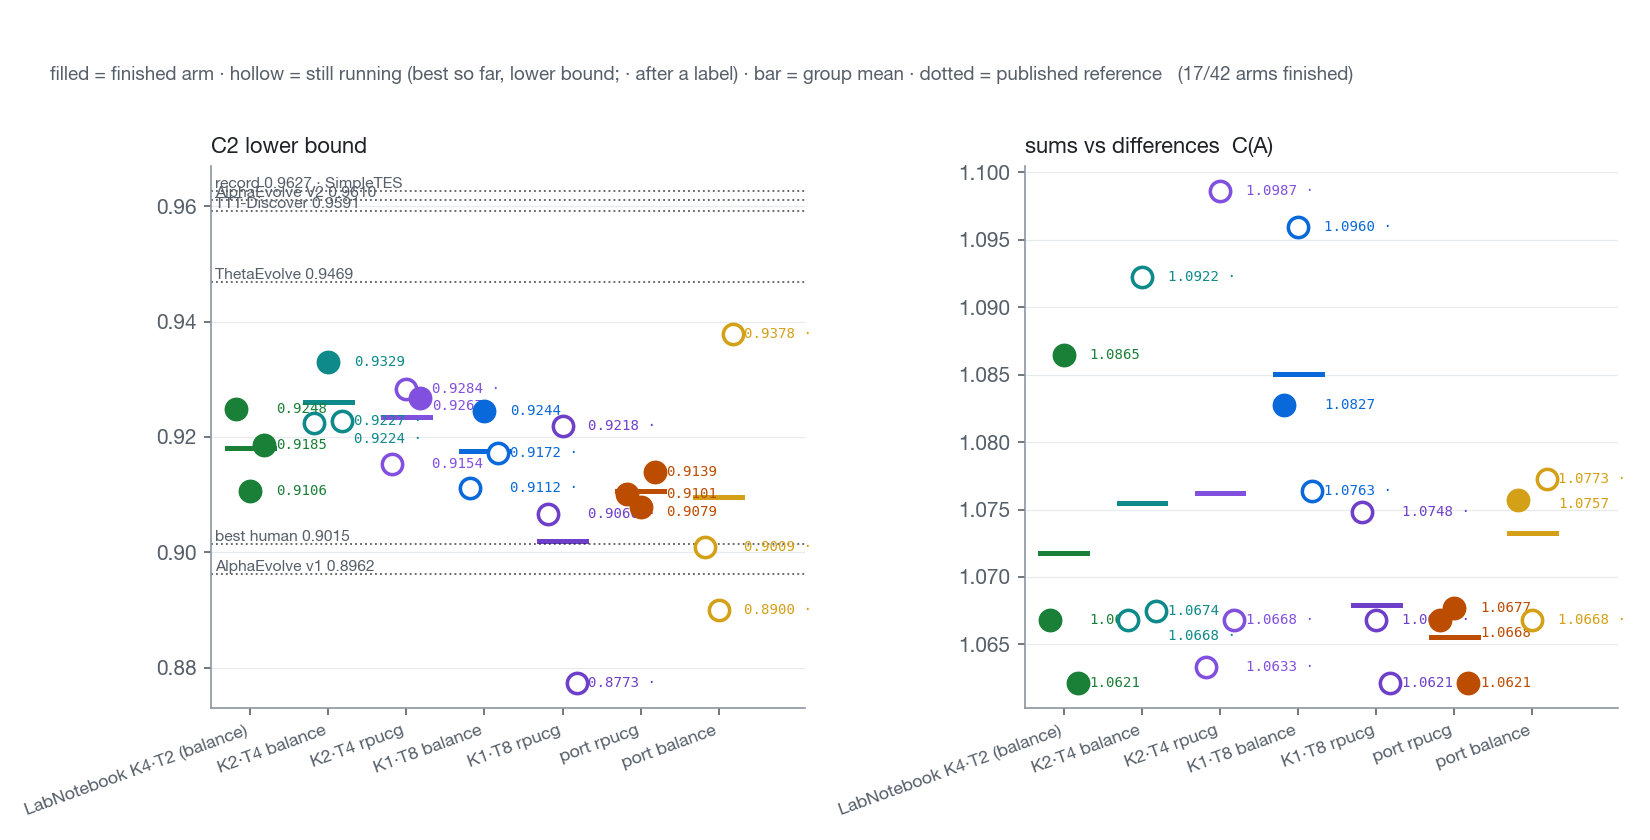
\includegraphics[width=\textwidth]{lab_notebook_figs/part3_selector.png}
\caption{Selector study, final. No consistent winner between the selectors: at $K{=}2$, $T{=}4$
balance leads on C2 (0.9268 against 0.9198) and rpucg on sums vs differences (1.0955 against
1.0785), both gaps inside about two replicate spreads. What is consistent is the trajectory length:
every $T{\ge}4$ cell beats the full method's $K{=}4$, $T{=}2$ on both tasks, and the single best
sums-vs-differences value of the whole program (1.1116) came from $K{=}1$, $T{=}8$ with rpucg.}
\label{fig:sel}
\end{figure}


\subsection{LabNotebook against SimpleTES across every task}
\label{sec:headtohead}

Table~\ref{tab:h2h} collects the two methods' results on every main-campaign task (Sections~3--8.5),
as the mean of three seeds of the bench's combined score (always maximised) with the seed range;
``clear'' means the ranges do not overlap. LabNotebook is at least as good on 17 of 22
task--campaign pairs and better where the search is open: all three AHC039 campaigns (the only clear,
repeatable gap, +21, +52 and +40 points, every pro LabNotebook arm above every port arm), hexagon-11, and
leaning on C2, Heilbronn-13, sums vs differences and AHC046. It loses clearly on Hadamard-29 and
AHC026, and leans behind on C3, kissing-11 and AHC058. Ten pairs are ties,
mostly because both methods reach the known optimum (packing, Erd\H{o}s, min--max) or sit inside
replicate spread.

\begin{table}[H]\centering\small
\caption{LabNotebook vs our SimpleTES port on every main-campaign task: mean of three seeds
[min, max] of the combined score, higher is better. Campaigns: \emph{flash} = deepseek-v4-flash on the
three original tasks (Sections~3--5), \emph{pro} = deepseek-v4-pro on the same tasks (Section~6),
\emph{AE} = the twelve AlphaEvolve-suite problems, batches A--D, on deepseek-v4-flash
(Sections~8.1--8.5); \emph{v4.1} = the Sherlock blocks on deepseek-v4.1-flash without thinking
(Tables~\ref{tab:part2} and \ref{tab:abld}; the LabNotebook and port rows of those blocks).}
\label{tab:h2h}
\begin{tabular}{@{}llrrrl@{}}
\toprule
campaign & task & LabNotebook & SimpleTES & $\Delta$ & reading \\
\midrule
flash & AHC039 & \textbf{2.4886} [2.481, 2.496] & 2.4743 [2.467, 2.482] & +0.6\% & LabNotebook, near-clear \\
flash & circle packing 26 & \textbf{2.6360} [record $\times$3] & 2.6349 [2.634, 2.636] & +0.04\% & both at the record \\
flash & Erd\H{o}s & 0.6188 & 0.6186 & +0.04\% & tie (barrier) \\
pro & AHC039 & \textbf{2.5071} [2.498, 2.517] & 2.4727 [2.469, 2.475] & +1.4\% & LabNotebook, clear \\
pro & circle packing 26 & 2.6354 & 2.6354 & 0 & tie \\
pro & Erd\H{o}s & 0.6189 & 0.6188 & 0 & tie \\
AE & $C_1$ & 0.6618 & 0.6620 & $-$0.02\% & tie \\
AE & $C_2$ & \textbf{0.9180} [0.911, 0.925] & 0.9106 [0.908, 0.914] & +0.8\% & LabNotebook, lean \\
AE & $C_3$ & 0.9880 & \textbf{0.9919} & $-$0.4\% & SimpleTES, lean \\
AE & circle packing 32 & 2.9396 [record $\times$3] & 2.9376 & +0.07\% & both at the record \\
AE & Hadamard 29 & 0.8165 [0.728, 0.862] & \textbf{0.8850} [0.860, 0.936] & $-$7.7\% & SimpleTES, clear \\
AE & Heilbronn convex 13 & \textbf{0.9142} [0.852, 1.000] & 0.8889 & +2.8\% & LabNotebook, lean \\
AE & Heilbronn triangle 11 & 0.8871 & 0.8847 & +0.3\% & tie \\
AE & hexagon 11 & \textbf{0.8522} [0.627, 0.983] & 0.4913 [$\times$3] & +73\% & LabNotebook, clear \\
AE & kissing 11 & 0.9770 & \textbf{0.9815} [$\times$3] & $-$0.5\% & SimpleTES, lean \\
AE & min--max 2D 16 & 0.9993 & 1.0000 & $-$0.07\% & tie (saturated) \\
AE & packing rect 21 & 0.9991 & 0.9947 & +0.4\% & tie \\
AE & sums vs differences & \textbf{1.0718} [1.062, 1.087] & 1.0655 & +0.6\% & LabNotebook, lean \\
v4.1 & AHC039 & \textbf{2.5031} [2.485, 2.525] & 2.4769 [2.461, 2.490] & +1.1\% & LabNotebook, near-clear \\
v4.1 & AHC058 & 5.2847 [5.159, 5.371] & \textbf{5.3274} [5.284, 5.364] & $-$0.8\% & SimpleTES, lean \\
v4.1 & AHC046 & \textbf{1.4303} [1.396, 1.451] & 1.4193 [1.361, 1.449] & +0.8\% & LabNotebook, lean \\
v4.1 & AHC026 & 0.9179 [0.915, 0.921] & \textbf{0.9258} [0.924, 0.927] & $-$0.8\% & SimpleTES, clear \\
\bottomrule
\end{tabular}
\end{table}


\begin{table}[H]\centering\small
\caption{LLM spend behind Table~\ref{tab:h2h}: mean tokens (prompt + completion, millions) and calls
per arm, and the recorded OpenRouter spend where both methods have it (the flash campaign's
SimpleTES arms predate spend recording). Two budget regimes: the AlphaEvolve suite, circle packing
and Erd\H{o}s arms stop on a 3.5M-token budget, so both methods spend about the same tokens and
LabNotebook simply makes more, shorter calls; the AHC039 arms stop on a 480-call budget, and there
LabNotebook spends 30--40\% fewer tokens (its idea and digest calls are short, the port emits two
full candidates per call) while scoring higher. The v4.1 blocks repeat the token pattern (AHC039
half the port's tokens and spend, AHC058 a quarter fewer, AHC046 equal tokens at 40\% less spend,
AHC026 40\% fewer tokens and spend) without the score advantage on AHC058 and AHC026.}
\label{tab:h2hcost}
\begin{tabular}{@{}llrrrrl@{}}
\toprule
campaign & task & LN Mtok & SimpleTES Mtok & LN calls & SimpleTES calls & recorded \$ LN / SimpleTES \\
\midrule
flash & AHC039 & \textbf{17.4} & 25.8 & 482 & 481 & 3.08 / --- \\
flash & circle packing 26 & 3.40 & 3.38 & 152 & 104 & 0.67 / --- \\
flash & Erd\H{o}s & 3.50 & 2.73 & 157 & 77 & 0.68 / --- \\
pro & AHC039 & \textbf{20.4} & 35.0 & 481 & 481 & \textbf{34.5} / 57.2 \\
pro & circle packing 26 & 3.30 & 3.57 & 140 & 94 & 7.5 / 7.9 \\
pro & Erd\H{o}s & 3.52 & 3.58 & 147 & 86 & 9.0 / 9.4 \\
AE & $C_1$ & 2.23 & 2.64 & 92 & 90 & 0.57 / 0.50 \\
AE & $C_2$ & 2.25 & 3.15 & 84 & 109 & 0.49 / 0.64 \\
AE & $C_3$ & 3.55 & 3.53 & 121 & 76 & 0.78 / 0.78 \\
AE & circle packing 32 & 3.54 & 3.56 & 136 & 97 & 0.84 / 0.60 \\
AE & Hadamard 29 & 3.53 & 3.41 & 104 & 90 & 0.63 / 0.67 \\
AE & Heilbronn convex 13 & 3.62 & 3.56 & 122 & 69 & 0.76 / 0.42 \\
AE & Heilbronn triangle 11 & 3.56 & 1.74 & 113 & 102 & 0.76 / 0.23 \\
AE & hexagon 11 & 3.57 & 3.74 & 84 & 60 & 0.70 / 0.40 \\
AE & kissing 11 & 3.62 & 3.21 & 90 & 88 & 0.76 / 0.82 \\
AE & min--max 2D 16 & 3.55 & 3.52 & 109 & 84 & 0.69 / 0.67 \\
AE & packing rect 21 & 3.54 & 3.59 & 98 & 65 & 0.73 / 0.42 \\
AE & sums vs differences & 3.63 & 3.56 & 98 & 85 & 0.83 / 0.81 \\
v4.1 & AHC039 & \textbf{15.2} & 30.4 & 482 & 481 & \textbf{7.82} / 14.33 \\
v4.1 & AHC058 & \textbf{4.9} & 6.8 & 483 & 480 & \textbf{2.29} / 2.96 \\
v4.1 & AHC046 & 5.8 & 5.8 & 482 & 480 & \textbf{1.29} / 2.14 \\
v4.1 & AHC026 & \textbf{3.6} & 6.3 & 483 & 480 & \textbf{0.83} / 1.43 \\
\bottomrule
\end{tabular}
\end{table}

\subsection{Reading the results}

\begin{itemize}
\item \textbf{Where the idea loop pays: the open-ended task.} On AHC039 all six LabNotebook arms
  beat every arm of every other method, with both models; the pro arms average 45 points above the
  next method. This is the task whose search space is structured enough that scoring an
  \emph{idea} by the best of a short local search, and keeping a notebook of what has been tried,
  changes what gets explored. It is not every AtCoder task: on AHC058, AHC046 and AHC026
  (Table~\ref{tab:abld}) the same block gives the port the lead on two (clearly on AHC026) and the
  no-ideas variant on the third.
\item \textbf{Where it is a tie: known optima.} Circle packing and Erd\H{o}s reduce to finding a
  known local optimum; once the inner optimizer is right, every method lands on it. LabNotebook is
  never worse and its replicates are tighter (3/3 record on flash packing against SimpleTES's 1/3;
  pro Erd\H{o}s within 0.00006), which in practice means fewer wasted runs.
\item \textbf{Where SimpleTES is better: exploiting an incumbent.} Under a warm start SimpleTES
  improves on every seed and LabNotebook gets worse on two of three. The fix is cheap
  ($p_{\text{best}}\to1$ and a smaller $K$ when a warm start is present) but has not been run.
\item \textbf{AlphaEvolve suite.} Batch A: packing $n{=}32$ LabNotebook on the record 3/3, SimpleTES
  2/3; $C_2$ LabNotebook's on every replicate; $C_1$ a tie. Batch B: sums vs differences LabNotebook's
  (best single and mean); $C_3$ a tie (SimpleTES by 0.006 in the mean); Hadamard-29 SimpleTES's
  (0.885 vs 0.817). Batch C: kissing-11 and Heilbronn-triangle ties; Heilbronn-convex LabNotebook's
  (0.914 vs 0.889, one arm at AlphaEvolve's value). Batch D: min/max-16 and rectangle-packing-21
  ties at AlphaEvolve's value; hexagon-11 HypothesisBandit's (0.957), LabNotebook second (0.852),
  SimpleTES unable to produce a program --- its whole-program completion fails on a long seed, a
  weakness LabNotebook shares only partially (it uses the same operator, but its ideas steer
  shorter rewrites). Across all twelve tasks: LabNotebook ahead of SimpleTES on five, SimpleTES on
  one, six ties --- and both far ahead of the two agent-based methods on all but hexagon-11. All
  are behind the 2026 systems by margins their extra compute explains.
\item \textbf{What the ablations attribute the effect to.} On the five tasks with a full block
  (Tables~\ref{tab:part2}, \ref{tab:ablc}, \ref{tab:abld}) only the ideas and the parallel short
  trajectories move the score beyond seed noise, and only on AHC039 and the two geometry tasks; the
  prose notebook and the digest are within noise on four tasks and hurt on hexagon-11, and the arm
  with no memory at all (ideas from the parent program alone) matches or beats the full method on
  both geometry tasks. On AHC058, AHC046
  and AHC026 no LabNotebook variant separates from another; the port leads two of the three, and the
  full method evaluates about a quarter fewer candidates than the port under the shared call budget.
\item \textbf{Limits of the evidence.} Three arms per cell and model sampling unseeded, so
  differences inside a group's seed spread (most of Tables~\ref{tab:ablc} and \ref{tab:abld}) are
  not resolved; the no-memory arm (Table~\ref{tab:ablc}) is the one that removes every learned
  input to the proposer, and it loses nothing.
\end{itemize}
